\title{誰が炎上させるのか}
\author{プロジェクトマネジメントコース\\
ソフトウェア開発管理グループ\\
矢吹研究室\\	
1342069\\
下村 渉}
\date{}
\begin{document}
\maketitle

%本テンプレートの余白は,卒論マニュアルで指示されたものとは違っているが,1ページあたりの文字数は40文字x40行と,卒論マニュアル通りになっている。文字間隔や行間隔を調整して,余白をマニュアル通りにすることもできるが,それでは文章が読みにくくなるため,このような対応をしている。

%\noindent
□□□□□□□□□■□□□□□□□□□■□□□□□□□□□■□□□□□□□□□■
□□□□□□□□□■□□□□□□□□□■□□□□□□□□□■□□□□□□□□□■
□□□□□□□□□■□□□□□□□□□■□□□□□□□□□■□□□□□□□□□■
□□□□□□□□□■□□□□□□□□□■□□□□□□□□□■□□□□□□□□□■
□□□□□□□□□■□□□□□□□□□■□□□□□□□□□■□□□□□□□□□■
□□□□□□□□□■□□□□□□□□□■□□□□□□□□□■□□□□□□□□□■
□□□□□□□□□■□□□□□□□□□■□□□□□□□□□■□□□□□□□□□■
□□□□□□□□□■□□□□□□□□□■□□□□□□□□□■□□□□□□□□□■
□□□□□□□□□■□□□□□□□□□■□□□□□□□□□■□□□□□□□□□■
□□□□□□□□□■□□□□□□□□□■□□□□□□□□□■□□□□□□□□□■
□□□□□□□□□■□□□□□□□□□■□□□□□□□□□■□□□□□□□□□■
□□□□□□□□□■□□□□□□□□□■□□□□□□□□□■□□□□□□□□□■
□□□□□□□□□■□□□□□□□□□■□□□□□□□□□■□□□□□□□□□■
□□□□□□□□□■□□□□□□□□□■□□□□□□□□□■□□□□□□□□□■
□□□□□□□□□■□□□□□□□□□■□□□□□□□□□■□□□□□□□□□■
□□□□□□□□□■□□□□□□□□□■□□□□□□□□□■□□□□□□□□□■
□□□□□□□□□■□□□□□□□□□■□□□□□□□□□■□□□□□□□□□■
□□□□□□□□□■□□□□□□□□□■□□□□□□□□□■□□□□□□□□□■
□□□□□□□□□■□□□□□□□□□■□□□□□□□□□■□□□□□□□□□■
□□□□□□□□□■□□□□□□□□□■□□□□□□□□□■□□□□□□□□□■
□□□□□□□□□■□□□□□□□□□■□□□□□□□□□■□□□□□□□□□■
□□□□□□□□□■□□□□□□□□□■□□□□□□□□□■□□□□□□□□□■
□□□□□□□□□■□□□□□□□□□■□□□□□□□□□■□□□□□□□□□■
□□□□□□□□□■□□□□□□□□□■□□□□□□□□□■□□□□□□□□□■
□□□□□□□□□■□□□□□□□□□■□□□□□□□□□■□□□□□□□□□■
□□□□□□□□□■□□□□□□□□□■□□□□□□□□□■□□□□□□□□□■
□□□□□□□□□■□□□□□□□□□■□□□□□□□□□■□□□□□□□□□■
□□□□□□□□□■□□□□□□□□□■□□□□□□□□□■□□□□□□□□□■
□□□□□□□□□■□□□□□□□□□■□□□□□□□□□■□□□□□□□□□■
□□□□□□□□□■□□□□□□□□□■□□□□□□□□□■□□□□□□□□□■
□□□□□□□□□■□□□□□□□□□■□□□□□□□□□■□□□□□□□□□■
□□□□□□□□□■□□□□□□□□□■□□□□□□□□□■□□□□□□□□□■
□□□□□□□□□■□□□□□□□□□■□□□□□□□□□■□□□□□□□□□■
□□□□□□□□□■□□□□□□□□□■□□□□□□□□□■□□□□□□□□□■
□□□□□□□□□■□□□□□□□□□■□□□□□□□□□■□□□□□□□□□■
□□□□□□□□□■□□□□□□□□□■□□□□□□□□□■□□□□□□□□□■
□□□□□□□□□■□□□□□□□□□■□□□□□□□□□■□□□□□□□□□■
□□□□□□□□□■□□□□□□□□□■□□□□□□□□□■□□□□□□□□□■
□□□□□□□□□■□□□□□□□□□■□□□□□□□□□■□□□□□□□□□■
■■■■■■■■■■■■■■■■■■■■■■■■■■■■■■■■■■■■■■■■
□□□□□□□□□■□□□□□□□□□■□□□□□□□□□■□□□□□□□□□■%文字数チェック用

\tableofcontents%目次





\chapter{背景}
ネットサービスが急速な発展をし,ソーシャルメディアを利用すれば,不特定多数の相手に対して,個人が情報を発信することも容易になっている.しかし,ネット上でのコミュニケーションが活発になる一方で,ある人物が発言した内容や行った行為について,ソーシャルメディアに批判的なコメントが殺到する現象「ネット炎上」が多発するようになってきている\cite{a}.炎上が日本で認識されるようになったのは2004年に無料ブログやSNSが多くサービスを開始したこととされ,2011年頃から顕著に増加している\cite{b}.

 短文の投稿を共有するウェブ上の情報サービスであるTwitterでは日常的に悪質なツイートがされる.例えば一般ユーザーがファッションセンターしまむらの店員に対し土下座を強要し,その光景を写真に収めツイートした件やコンビニエンスストアであるローソンの従業員がアイスケースの中に入った写真をツイートした件などがある.

日常的に悪質なツイートがされることに対し,悪ふざけや犯罪を自慢するツイート,情報モラル,情報リテラシーが低いツイートを見過ごさず,通報やリツイートをする正義感溢れる人達がいる.彼らはそれ相応の罰を受ける必要があるという気持ちや何度も同じ過ちを繰り返してしまわないようにという正義感から通報やリツイートをする.リツイート数が伸びると便乗してリツイートするユーザが増え,結果事態が大きくなってしまい炎上してしまう場合がある.
 
\chapter{目的}
本研究の目的はTwitter上で悪ふざけの投稿や犯罪自慢投稿,情報モラル,リテラシーの低いツイートをより多くリツイートしているユーザの特定し,炎上のリスク対策ができるような指標を作成する.
\chapter{手法}

\section{本章の構成}
本章では研究方法について説明する.
\section{研究方法}

VirtualBoxをインストールして仮想マシンを作成し,そこにUbuntuをインストールする.その後,Ubuntu上でPythonとTweepyをインストールして,TwitterとStreaming APIを使用しデータの集計をする.Streamingデータから,リツイートだけを取り出し,データベースに格納する.リツイートした人,された人のフォロー関係を調べ,データベースに記録する.

\chapter{Twitterについて}


\section{本章の構成}
本章では本研究で使用するTwitterについて説明する.

\section{Twitterとは}
Twitter(ツイッター)は,「ツイート」と称される140文字以内の短文の投稿を共有するWEB上の情報サービスである.Twitterに発言を投稿するにはパソコンや携帯電話,スマートフォンで自身のアカウントにログインし,画面上部のボックスに内容を入力し「ツイート」ボタンを押すことで投稿が完了する.タイムラインと呼ばれる画面には,自分のつぶやきとフォローしたユーザのツイートが同一画面上に,リアルタイムで表示される.相手がツイートを非公開にしていなければ,フォローをする際の承認は不要で,ツイートを引用することもできる.ツイートやユーザの検索をすることも可能で,ユーザ同士がつながる機会は多岐にわたる.



\section{用語}
本節では,本研究で利用するTwitterの用語について説明する.

\subsection{ユーザー名}
ユーザー名とは半角英数字,アンダーバーから計15文字以内で作る,TwitterでのIDラベルである.

\clearpage
\begin{figure}[htb]
\centering

\includegraphics[width=15cm]{twitter.png}
\caption{twitterサイト}\label{twitter}
\end{figure}
\subsection{プロフィールページ}
http://twitter.com/(ユーザー名) のWebページには自己紹介情報として,名前,プロフィール画像,バナー画像,自己紹介,Webサイト,場所,誕生日などを設定できる.これらを総称して「プロフィール」と呼ぶ.

\subsection{タイムライン}
自分とフォロー(後述)しているユーザのツイートがリアルタイムに,時系列に沿って表示される画面.この画面がTwitterでは基本となるため,「ホーム」とも呼ぶ.

\subsection{ツイート}
Twitterにおける「つぶやき」のこと.1つのツイートにつき160文字まで,という制限が設けられている.ただし,そのうちの20文字はユーザIDに割り当てられているため,残りの140文字がツイートの本文ということになる.

\clearpage
\begin{figure}[htb]
\centering
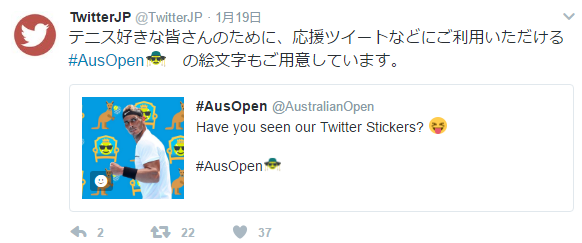
\includegraphics[width=15cm]{tweet.png}
\caption{ツイート}\label{ツイート}
\end{figure}

\subsection{リプライ}
他のユーザーに宛てたツイート.「@ユーザー名(投稿したい内容)」の書式で投稿すると,そのユーザー宛の返信扱いとなる.自分宛の投稿は一覧ページで確認することができる.ツイートの最初に@ユーザー名を入力して投稿すると,投稿をしたユーザーとされたユーザーのどちらか片方のみをフォローしている第三者ユーザーのタイムラインには表示されないが,双方をフォローしているユーザーのタイムラインには表示される.

\begin{figure}[htb]
\centering

\includegraphics[width=15cm]{reply.png}
\caption{リプライ}\label{reply}
\end{figure}
\clearpage
\subsection{いいね}
あとで読み返したいと思ったツイートや気に入ったツイートを,(♡)を付けて自分のいいねリストへ登録すること.以前はお気に入り (Favorites) だったが,2015年11月4日,「いいね」に変更され,これまでの「☆」から「♡」に変更された.

\subsection{リツイート}
他の人のツイートを再びツイートするというもの.自分のタイムラインに流れてきたツイートをリツイートすると,自分のフォロワーのタイムラインにそのツイートが流れる.逆に自分がフォローしているユーザーがリツイートすれば,自分のタイムラインにそのツイートが流れる.
\begin{figure}[htb]
\centering
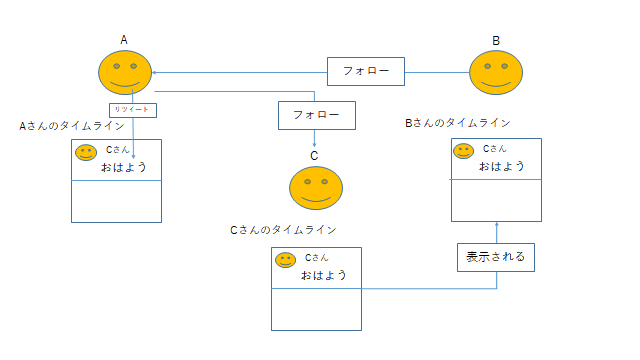
\includegraphics[width=15cm]{retweet.png}
\caption{リツイート}\label{retweet}
\end{figure}
\subsection{フォロー}

フォローボタンを押しユーザーをフォローすることによって,自分のタイムラインにそのユーザーのつぶやきが表示されるようにする機能の事である.

\subsection{フォロワー}

自分をフォローしているユーザーの事である.フォロワーのタイムラインには自分(フォローされている人)のつぶやきが表示される.

\section{Twitter APIについて}
本研究ではTwitterから様々な情報を取得するためのプログラムを使用する.その際に必要となるのがTwitter APIである.本節では,Twitter APIに関する説明をする.

\subsection{API}
アプリケーションプログラムインターフェイス(Application Program Interface)の略で,プログラミングの際に使用できる命令や規約,関数等の集合のことを示す.ソフトウェア開発の際,いちから全てを作るより,APIを利用すればもともとあるプログラムを呼び出して,その機能を組み込んだソフトウェアを開発することができる。.
\subsection{Twitter API}
Twitter社が提供するサービス.WebサイトやアプリケーションなどからTwitterの機能を呼び出すことができ,ツイートの参照や検索等を行えるアプリケーション開発を行えるようになる.

\subsection{REST API}
Twitter APIのパラメータ(リソース)を指定し,特定のURLにHTTPでアクセスすると,JSON形式で記述されたメッセージがレスポンスされるシステム.これはツイートの更新や参照を行う際に使用する基本的なAPIとなる.ただし利用制限があり,15分以内に同じ機能を特定の回数利用すると,はじめにその機能を利用した時間から15分経過するまではその機能が利用できなくなる.

\subsection{Streaming API}
今回利用するAPI.タイムラインの変更をリアルタイムで自動に受け取ることができる.

\subsection{Access Token}
Webサービスを利用するために,認証局がユーザーを認証するために払い出した認証情報のことを指す.ここで言う認証局とはユーザーを認証する情報を保持しており,ユーザーを認証することができるWebサーバーで,Webサービスを提供しているWebサーバー,または,ユーザーを認証することができる第三者のWebサーバーなどを示す.

\section{VirtualBoxとは}
VirtualBoxとは,使用しているPC上に仮想的なPCを作成し,別のOSをインストール・実行できるオープンソースソフトウェアである.例えばVirtualBoxをインストールPCがWindowsだったとしてそのWindows上でSolaris/OpenSolaris,Linux等,様々なOSで利用することができる\cite{c}.

\begin{figure}[htb]
\centering
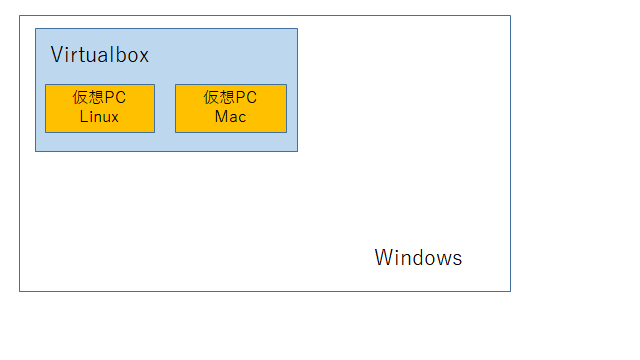
\includegraphics[width=15cm]{vbox.png}
\caption{vbox}\label{vbox}
\end{figure}

\section{用語}
本節では,本研究で利用するVirtualBoxの用語について説明する.


\subsection{OS}
OperationSystem(オペレーティング・システム)の略で,コンピューターを動かすためのソフトウェアのことである.コンピューター全体を管理,制御し,人が使えるようにする役割がある.
具体的には,キーボードやマウス・タッチパッドから入力した情報をアプリケーションに伝える役割を果たす,最も基本的なソフトウェアのことである.

\subsection{ホストOS}
仮想マシンのプログラムを動作させている基盤となるOSのこと.VirtualBoxはホストOSにインストールされる.

\subsection{仮想マシン}
VirtualBoxが作成する論理的なマシン.VirtualBoxがホストマシンのコンピュータ資源(CPUやメモリ,HDD等)の一部を仮想化し,ゲストマシンに割り当てる.ホストマシンの資源を使いきらない限り,ゲストマシンを複数作成したり,多重起動させることができる.例えば本来のコンピューターでは動作しないOSやソフトウエアを使かったり,実物を利用せずに携帯電話やゲーム機などのソフトウエアを試験するなどの様々な用途がある.

\subsection{ゲストOS}

ゲストOSとは,ひとつのコンピュータ上で別をコンピュータをエミュレートする「仮想マシン」と呼ばれる環境において,仮想マシン上で動いているOSのことである.
例えば,「仮想マシン」の環境を用意して,Windows上でLinuxを動かす場合,LinuxがゲストOSとなる.このとき,WindowsはホストOSと呼ばれる.
また,ゲストOSは,仮想マシンの環境からは,アプリケーションとして認識されるため,ゲストOSを動かすには,ホストOSの正常な状態が前提となる.ただし,ゲストOSに以上が生じても,仮想マシン環境そのものには影響はないため,仮想マシン環境を起動させたまま,ゲストOSを再起動させることが可能となっている.なお,仮想マシンを実現するソフトは,VirtualBoxやVMwareなどがある.

\subsection{仮想ディスク}
ゲストマシンが使用する仮想のハードディスク.バーチャルマシンからはこれを物理ディスクとして扱うことができる.仮想ディスクの実体はホストマシン内にファイルとして存在する.

\chapter{Ubuntuについて}

\section{本章の構成}

本章では本研究で使用するUbuntuについて説明する.

\section{Ubuntuとは}
UbuntuはLinuxのディストリビューション(配布形態)のひとつである.「Ubuntu」という名前はアフリカ・ズールー語で「他者への思いやり」を意味する.その名の通り,使いやすさに重点を置いており,他のディストリビューションと比べて簡単に使い始めることができる.

\subsection{「端末」とは}
Ubuntuをキーボード入力によるコマンドで操作するためのアプリケーション.「ターミナル」とも呼ばれる.Windowsでの「コマンド プロンプト」に相当する.

\subsection{VirtualBoxのインストール}

VirtualBoxのダウンロードサイト(http://www.oracle.com/technetwork/server-storage/virtualbox/downloads/index.html?ssSourceSiteId=otnjp)にアクセスし,Platformから自分のOSのインストーラーをダウンロードする.

\begin{figure}[htb]
\centering
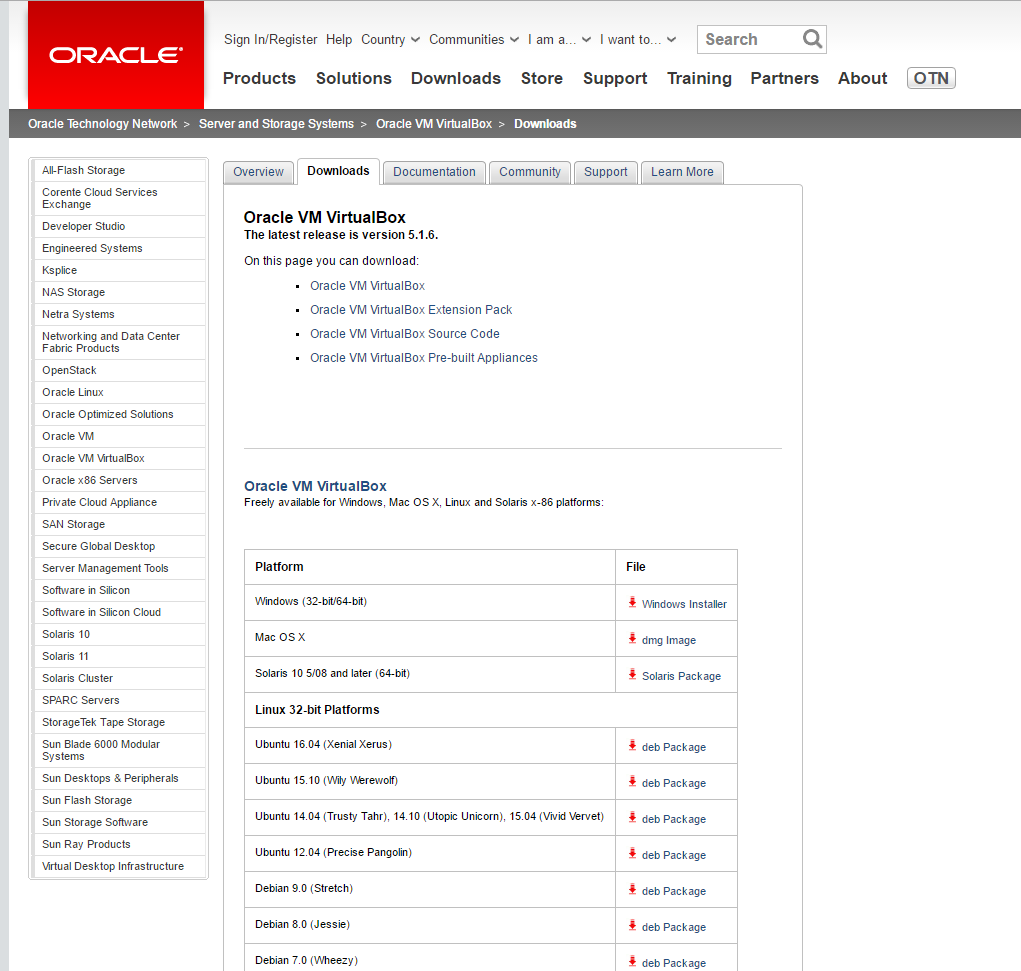
\includegraphics[width=15cm]{oracle.png}
\caption{ダウンロードサイト}\label{virtualboxダウンロードサイトの画像}
\end{figure}

\clearpage

インストーラーを起動し,セットアップウィザードを起動し,指示に従いインストールを開始する.
その後Warning Network Interfacesが表示されたら「Yes」をクリックする.

\begin{figure}[htb]
\centering
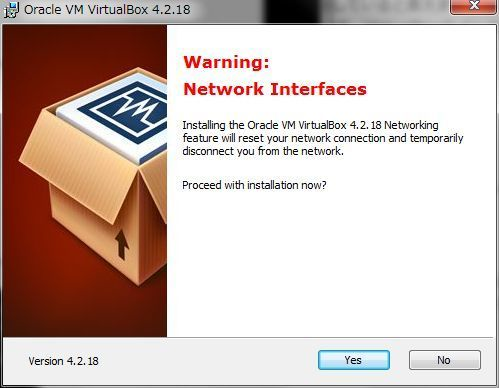
\includegraphics[width=15cm]{setup1.png}
\caption{インストール画面1}\label{virtualboxインストール画面1}
\end{figure}

\clearpage
Ready to Installが表示されたら「Install」をクリックする.
\begin{figure}[htb]
\centering
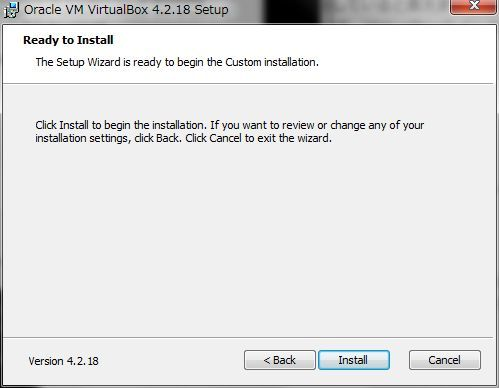
\includegraphics[width=15cm]{setup2.png}
\caption{インストール画面2}\label{virtualboxインストール画面2}
\end{figure}

インストール中にユーザーアカウント制御によってインストールを許可するか否かを聞いてくるが,「はい(Y)」をクリックする.

\clearpage
次に「Windows セキュリティ」ダイアログが表示されたら,「Oracle Corporationからのソフトウエアを常に信頼する(A)」をチェックし,
「インストール(I)」をクリックする.

\begin{figure}[htb]
\centering
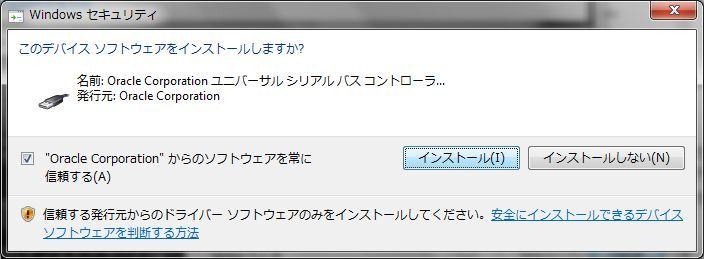
\includegraphics[width=15cm]{setup3.png}
\caption{インストール画面3}\label{virtualboxインストール画面3}
\end{figure}
インストールが終了すると,デスクトップ上にVirtualBoxのショートカットが作成され,インストールが完了する.


\clearpage


\subsection{Ubuntuのインストール}

UbuntuのISOデータを http://www.ubuntulinux.jp/ よりダウンロードする.
先ほどインストールしたVirtualBoxを起動し,仮想マシンの作成をする.

\begin{figure}[htb]
\centering
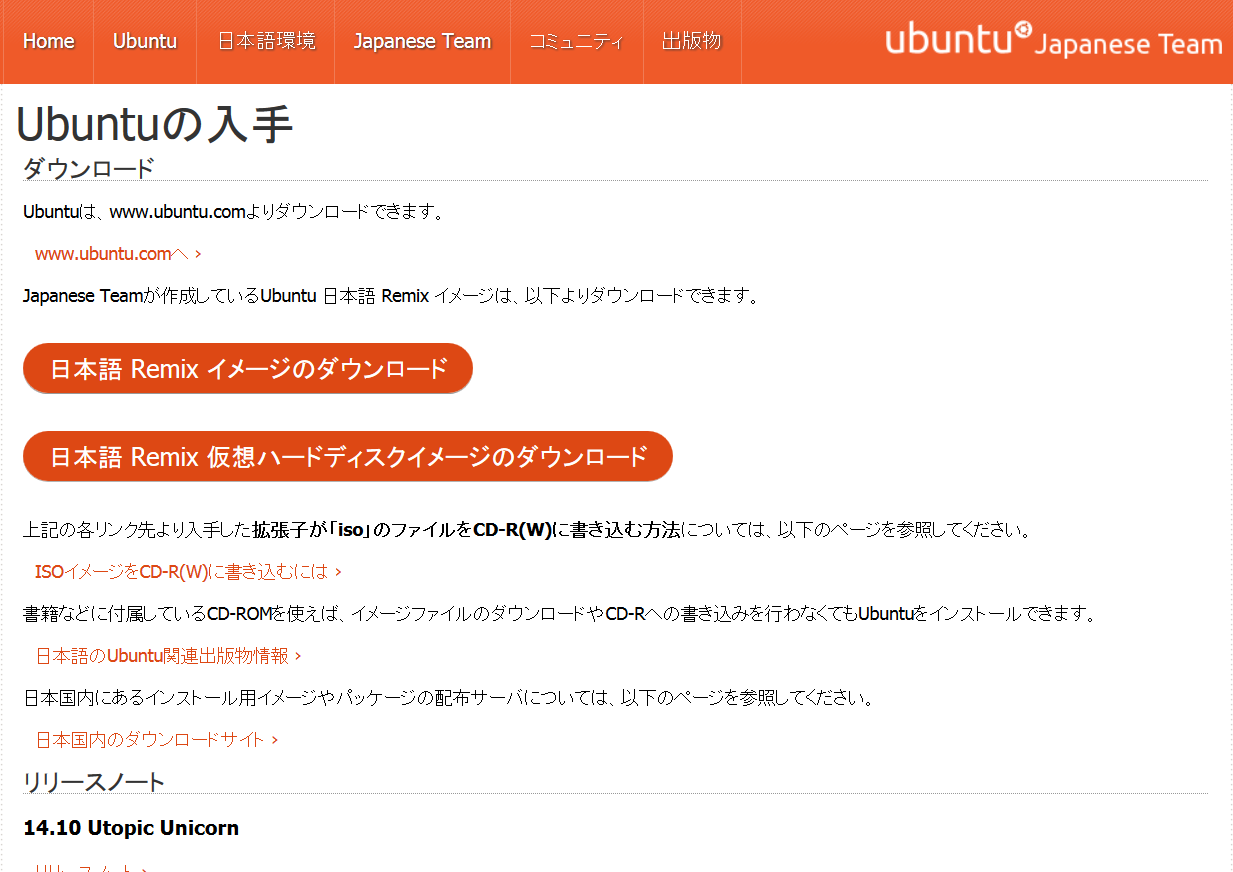
\includegraphics[width=15cm]{ubuntuinst.png}
\caption{Ubuntuのダウンロードページ}\label{Ubuntuのダウンロードページ}
\end{figure}

\clearpage

\subsection{仮想マシンの作成}

デスクトップ上のショートカットからVirtualBoxを起動する.その後VirtualBoxのホーム画面が表示されたら,「新規(N)」をクリックする.その後作成する仮想マシンの名前,メモリサイズ,仮想HDDの設定画面に移動する.

\begin{figure}[htb]
\centering
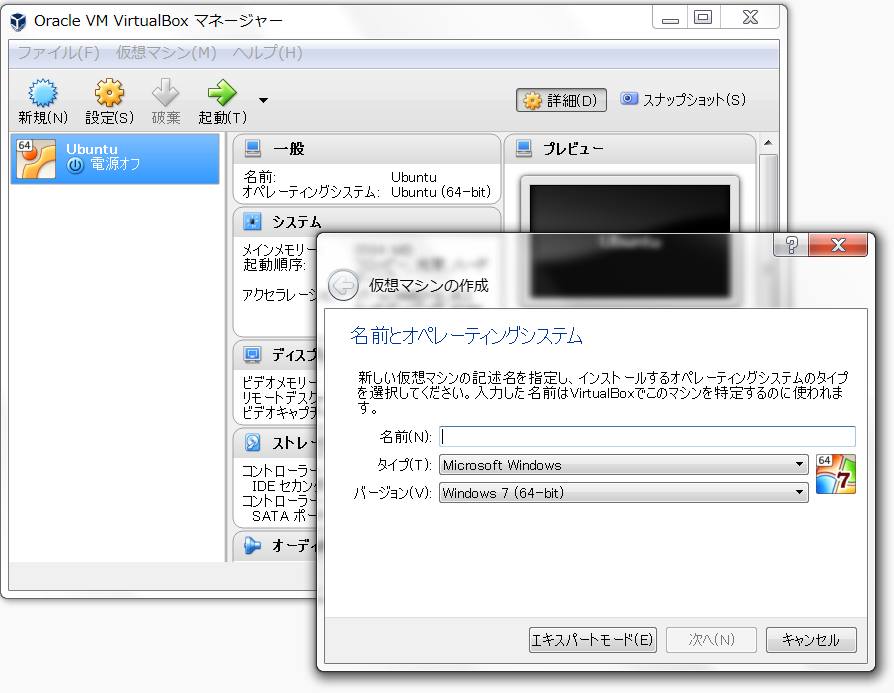
\includegraphics[width=15cm]{vb1.png}
\caption{仮想マシンの名前の設定画面}\label{仮想マシンの設定画面}
\end{figure}
\clearpage

仮想マシンのメモリサイズの設定は以下のように行う.設定後「次へ(N)」をクリックする.

\begin{figure}[htb]
\centering
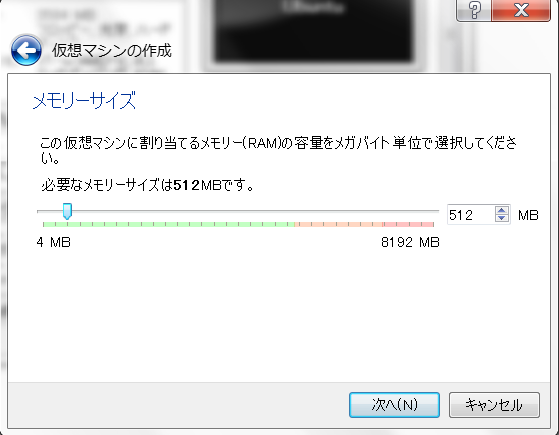
\includegraphics[width=15cm]{vb2.png}
\caption{仮想マシンのメモリサイズ設定画面}\label{仮想マシンの設定画面}
\end{figure}
\clearpage
仮想マシンの仮想HDDのファイルの形式を指定する.


\begin{figure}[htb]
\centering
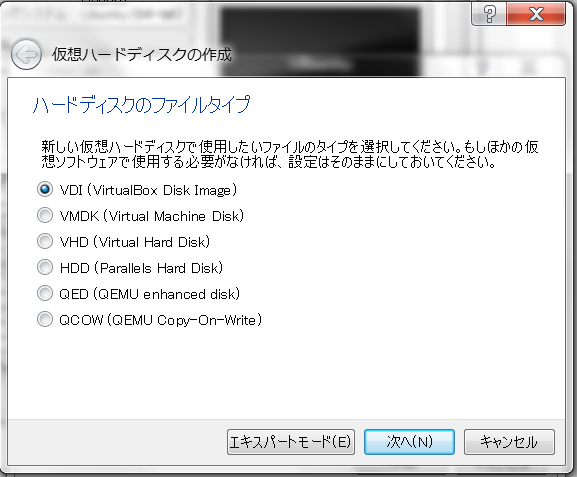
\includegraphics[width=15cm]{vb3.png}
\caption{仮想HDDのファイル形式作成画面}\label{仮想マシンの設定画面}
\end{figure}
\clearpage
作成するハードドライブのファイルの名前を指定する.



\begin{figure}[htb]
\centering
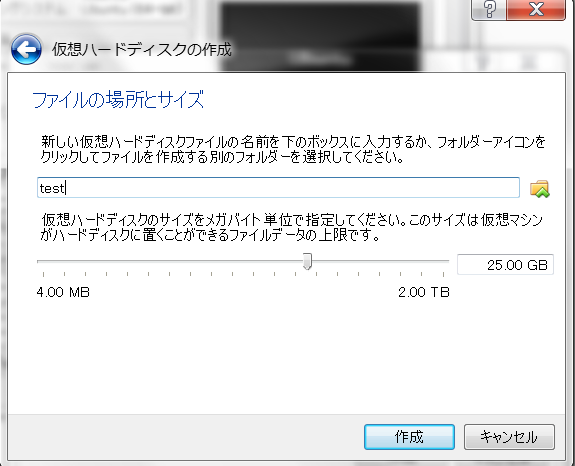
\includegraphics[width=15cm]{vb4.png}
\caption{仮想HDDの作成画面}\label{仮想マシンの設定画面}
\end{figure}
\clearpage
「作成」をクリックしたら以下の画面が表示され,仮想HDDが作成されると自動的にこの画面は閉じられる.


\begin{figure}[htb]
\centering
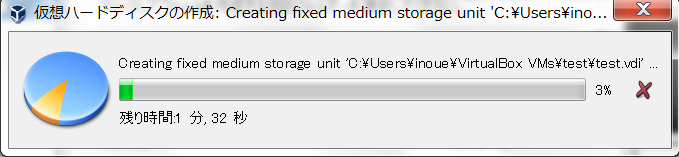
\includegraphics[width=15cm]{vb5.png}
\caption{仮想HDDの作成画面}\label{仮想マシンの設定画面}
\end{figure}

\clearpage


その後先ほど作成した仮想マシンを起動すると,インストール開始画面が表示される.

その後「設定(S)」をクリックし,「ストレージツリー(S)」の項目にある「空」選択する.さらに「属性」内にあるディスクのマークをクリックすると「仮想光学ディスクファイルを選択...」をクリックしUbuntuのISOイメージを選択する.

\begin{figure}[htb]
\centering
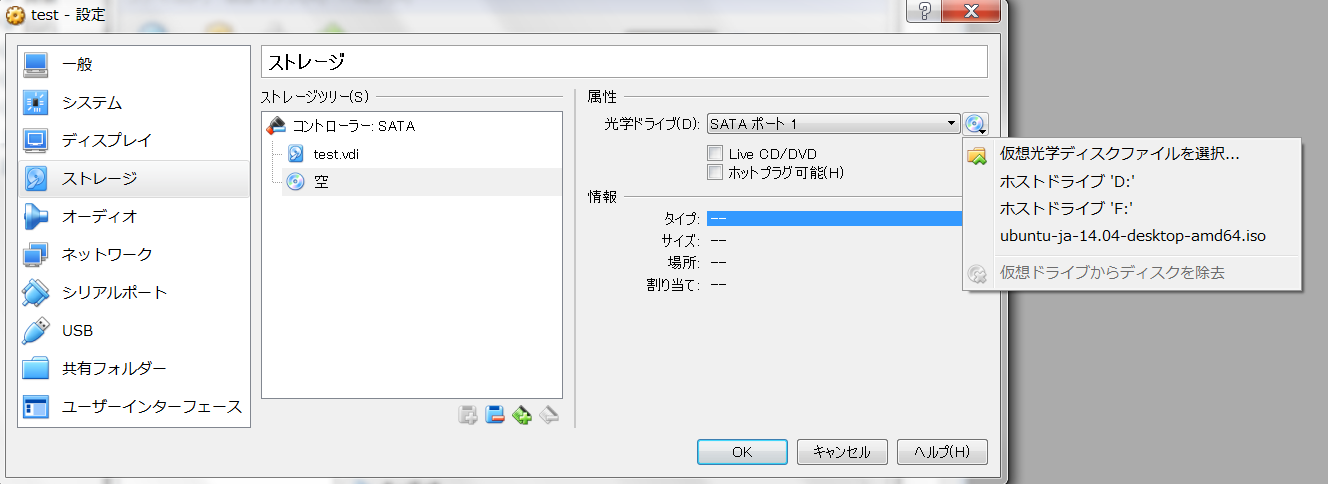
\includegraphics[width=15cm]{vb6.png}
\caption{ISOイメージ設定}\label{仮想マシンの設定画面}
\end{figure}

「OK」をクリックした後,仮想マシンを起動させると以下のような仮想マシン内でのインストールが始まる.

\begin{figure}[htb]
\centering
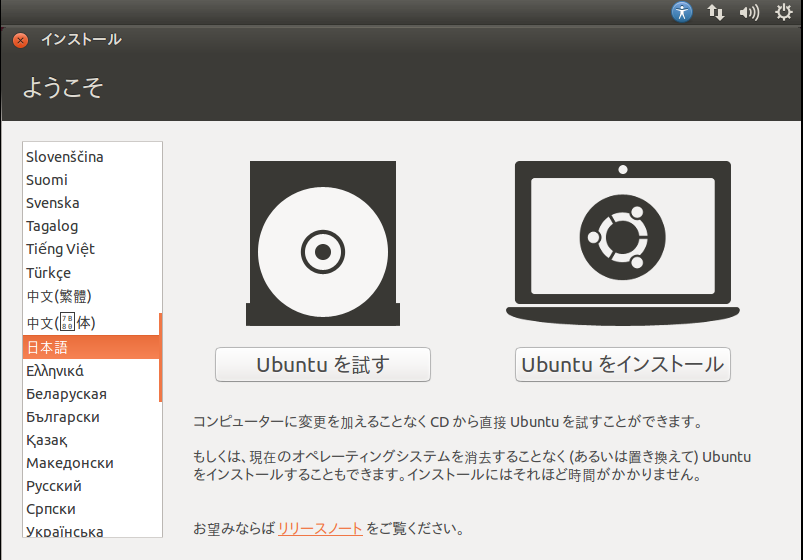
\includegraphics[width=15cm]{ubuntuinstall3.png}
\caption{インストール開始画面}\label{インストール開始画面}
\end{figure}

下の画面が出たら「Encrypt the new Ubuntu installation for security」,「Use LVM with the new Ubuntu installation」のチェックをはずし,「続ける」をクリックする
\begin{figure}[htb]
\centering
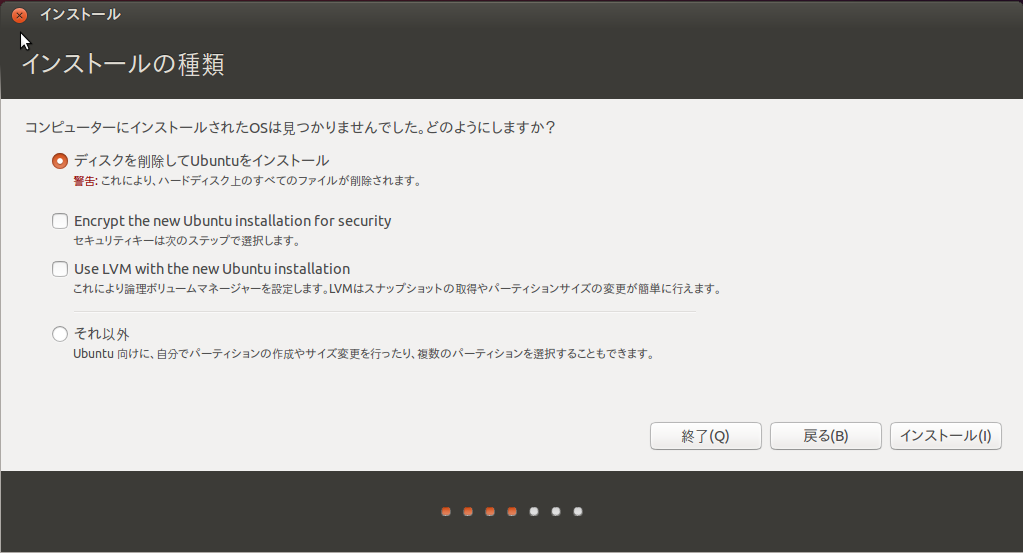
\includegraphics[width=15cm]{ubuntuinstall2.png}
\caption{インストール準備画面}\label{インストール準備画面}
\end{figure}

\clearpage
「インストール中にアップデートをダウンロードする」のチェックボックスにチェックを入れ,「続ける」をクリックする.
\begin{figure}[htb]
\centering
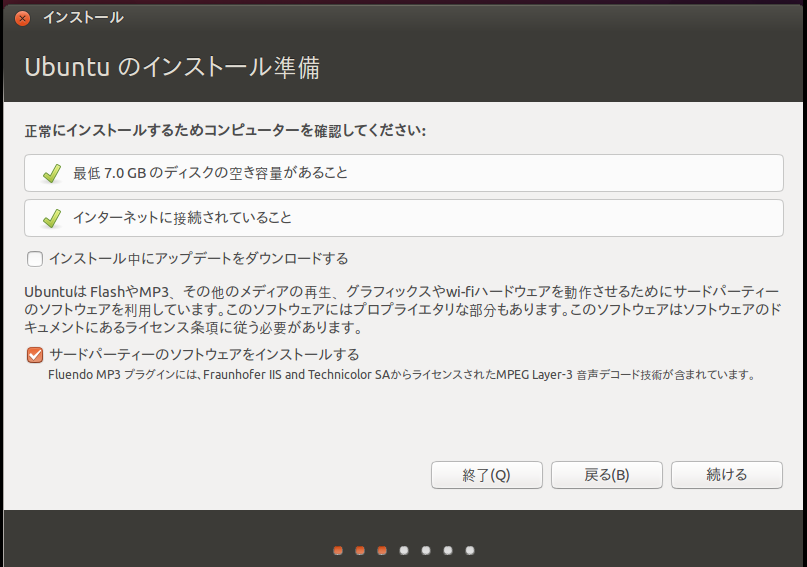
\includegraphics[width=15cm]{ubuntuinstall1.png}
\caption{インストールの種類}\label{インストール準備画面2}
\end{figure}
\clearpage
以下の画面でタイムゾーンを選択する.デフォルトで東京(Tokyo)が選択されているので,「続ける」をクリックする.

\begin{figure}[htb]
\centering
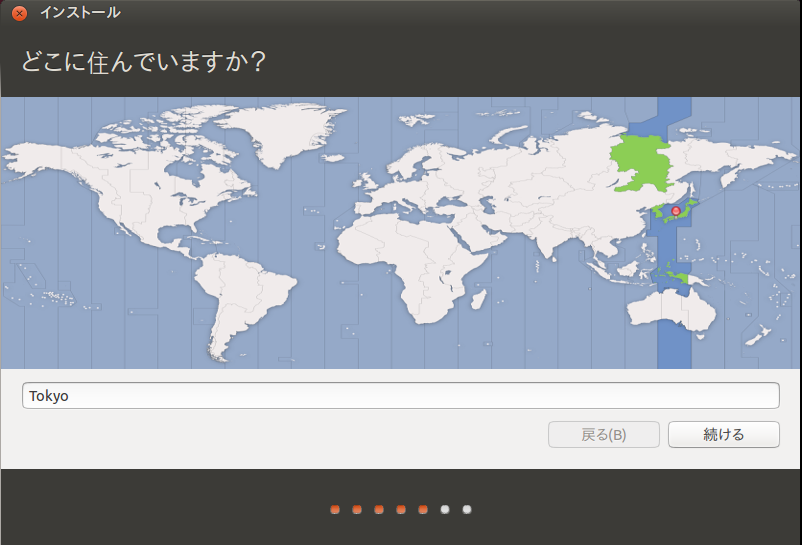
\includegraphics[width=15cm]{ubuntuinstall4.png}
\caption{タイムゾーン}\label{タイムゾーン}
\end{figure}
\clearpage

以下の画面でキーボード配列を選択する.そのまま「続ける」をクリックする.

\begin{figure}[htb]
\centering
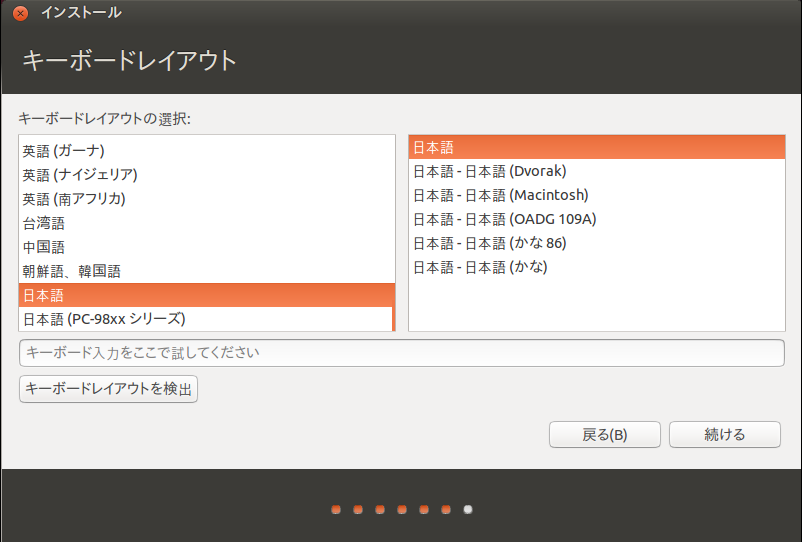
\includegraphics[width=15cm]{ubuntuinstall5.png}
\caption{キーボード配列}\label{キーボード配列}
\end{figure}
\clearpage

「あなたの名前」の欄には自分の名前を記載する.「コンピュータの名前」を適当に入力する.「ユーザー名の入力」は自分のユーザー名を決め,「パスワード」は任意で決める.それらの情報を入力したら「続ける」をクリックする.


\begin{figure}[htb]
\centering
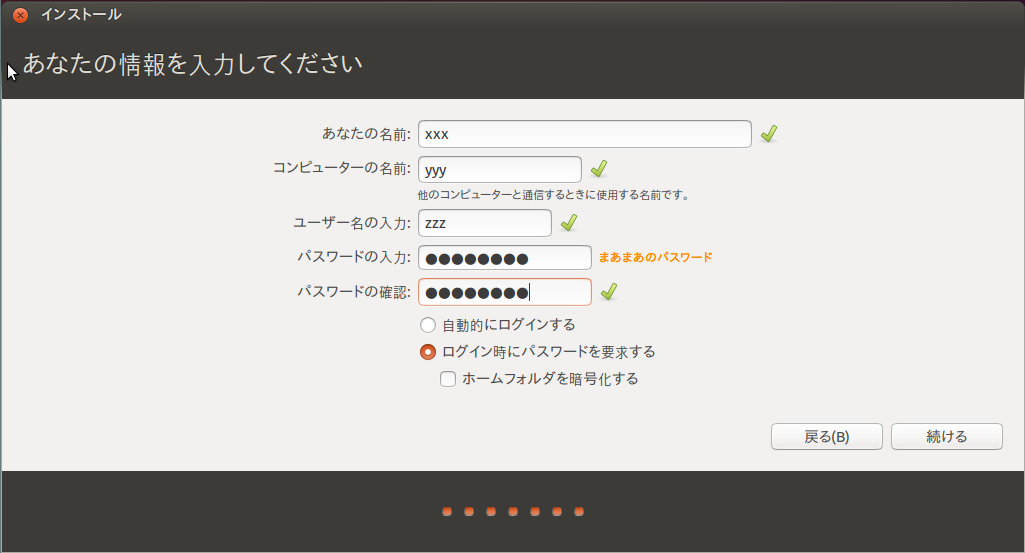
\includegraphics[width=15cm]{ubuntuinstall6.png}
\caption{情報入力画面}\label{情報入力画面}
\end{figure}

\clearpage
数分待機すると,インストールが終了し,以下の画面が表示される.「今すぐ再起動する」をクリックし,画面に表示されるメッセージがとまったら,何か適当かキーを打つ.すると,仮想マシンが再起動する.


\begin{figure}[htb]
\centering
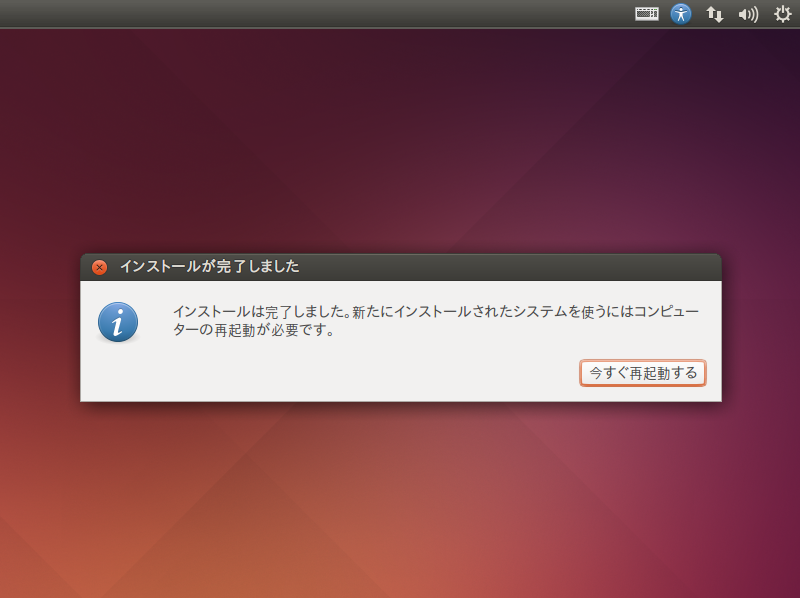
\includegraphics[width=15cm]{ubuntuinstall7.png}
\caption{インストール完了画面}\label{イメージ画面}
\end{figure}
\clearpage
この様な画面が表示されればインストールが終了する.


\begin{figure}[htb]
\centering
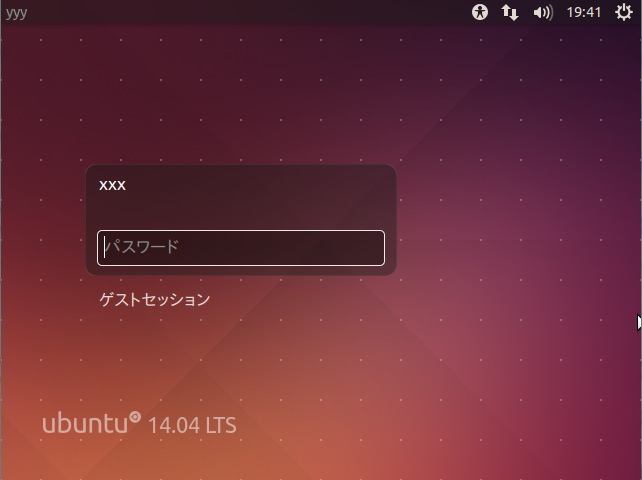
\includegraphics[width=15cm]{ubuntuinstall8.png}
\caption{ログイン画面}\label{イメージ画面}
\end{figure}
\clearpage


\chapter{Pythonについて}

\section{本章の構成}
本章では本研究で使用するプログラミング言語,Pythonについて記す.

\section{Pythonとは}
Pythonは,広く使用されている汎用のプログラミング言語であり,コードのリーダビリティが高くなるように言語が設計されていると言われ,その構文のおかげで,C言語に比べて,より少ないコード行数でプログラムを表現できると言われている.小規模なプログラムから大規模なプログラムまで,様々なプロ不ラムをクリアに書けるように,多くのコードが提供されている.
\subsection{Pythonの特徴}

Pythonには次のような特徴がある.

\subsubsection{文法がシンプル}
コードの読みやすさや書きやすさを重視しているので,文法もシンプルで必要最低限のものしか用意されていない.
そのため,プログラミング初心者にもわかりやすく,学びやすい言語である.
文法やシンプルだが機能は非常に強力で効率よく開発ができるので,生産性が非常に高い.

\subsubsection{専門分野に強い}
利便性の高い大規模な標準ライブラリが多数あります。
Pyhton言語自体は機能を最小限に抑えられているので,足りない部分はライブラリで機能を追加できるようになっている.
さまざまな分野に特化した大規模なライブラリが作られており,専用のアプリケーションでも簡単に作ることができる.
特に数学系のライブラリが充実しており,科学技術計算や統計解析などの分野に強く注目されている.

\clearpage

\section {Tweepyについて}
Tweepyとは,プログラム言語PythonでTwitterを利用するためのライブラリである.
Ubuntuなら次のように簡単にインストールできます.

\begin{verbatim}

sudo apt-get install python-setuptools python-pip
sudo easy_install tweepy

\end{verbatim}

コマンドを実行するとパスワードの入力を求められるので,パスワードを入力してEnterキーを押すとPythonとTweepyのインストールが開始される.
途中,続行しますかと尋ねられるので,「y」を入力し,Enterを押すとインストールが続行される.
\begin{figure}[htb]
\centering
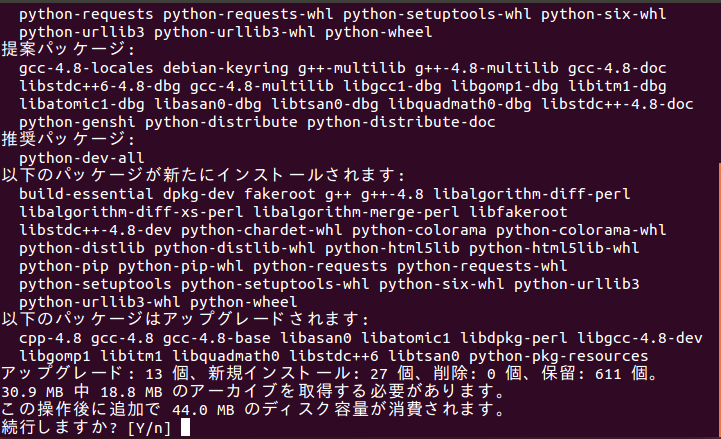
\includegraphics[width=15cm]{tweepy.png}
\caption{tweepy}\label{tweepy}
\end{figure}
\clearpage

\section{OAuth認証}
OAuthとは,Webサーバーにあるユーザーのリソースへのアクセス権限を,ユーザーの代理で行うことを許可するための認証用のプロトコルのことである.
OAuthを使用することで,エンドユーザーはクライアントにユーザ名やパスワードを知らせることなく,サーバーリソースへの第三者アクセスを認可することができる.OAuthでは,ログインのために必要なユーザー名とパスワードをユーザー毎に割り当てるトークンと呼ばれる情報に置き換えて使う.このトークンを使うことで外部のサービスにはパスワードを教えることなく,システム間の情報の共有が可能になる\cite{d}.また認可情報の適用範囲を指定したり,有効期限を設定することができるため,ユーザが外部サービスにすべての権限を渡すこと無く,自分が利用したいサービスに最低限必要な権限のみを委譲することができる.
\begin{verbatim}
# -*- coding: utf-8 -*-
import tweepy

consumer_key = ""
consumer_secret = ""

access_token = ""
access_token_secret = ""

auth = tweepy.OAuthHandler(consumer_key, consumer_secret)
auth.set_access_token(access_token, access_token_secret)
api = tweepy.API(auth)
\end{verbatim}

\clearpage

\section{アプリケーションの登録}
OAuthを使用するには,TwitterAPIで「Consumer key」,「Consumer Sercret」,「Access Token」,「Access Token Secret」の4つの情報を入手する必要がある.

\subsection{ユーザーアカウントの用意}
Twitter APIを利用するには,ユーザーアカウントが必要になるのでTwitter公式サイトでアカウント作成をクリックする.
\begin{figure}[htb]
\centering
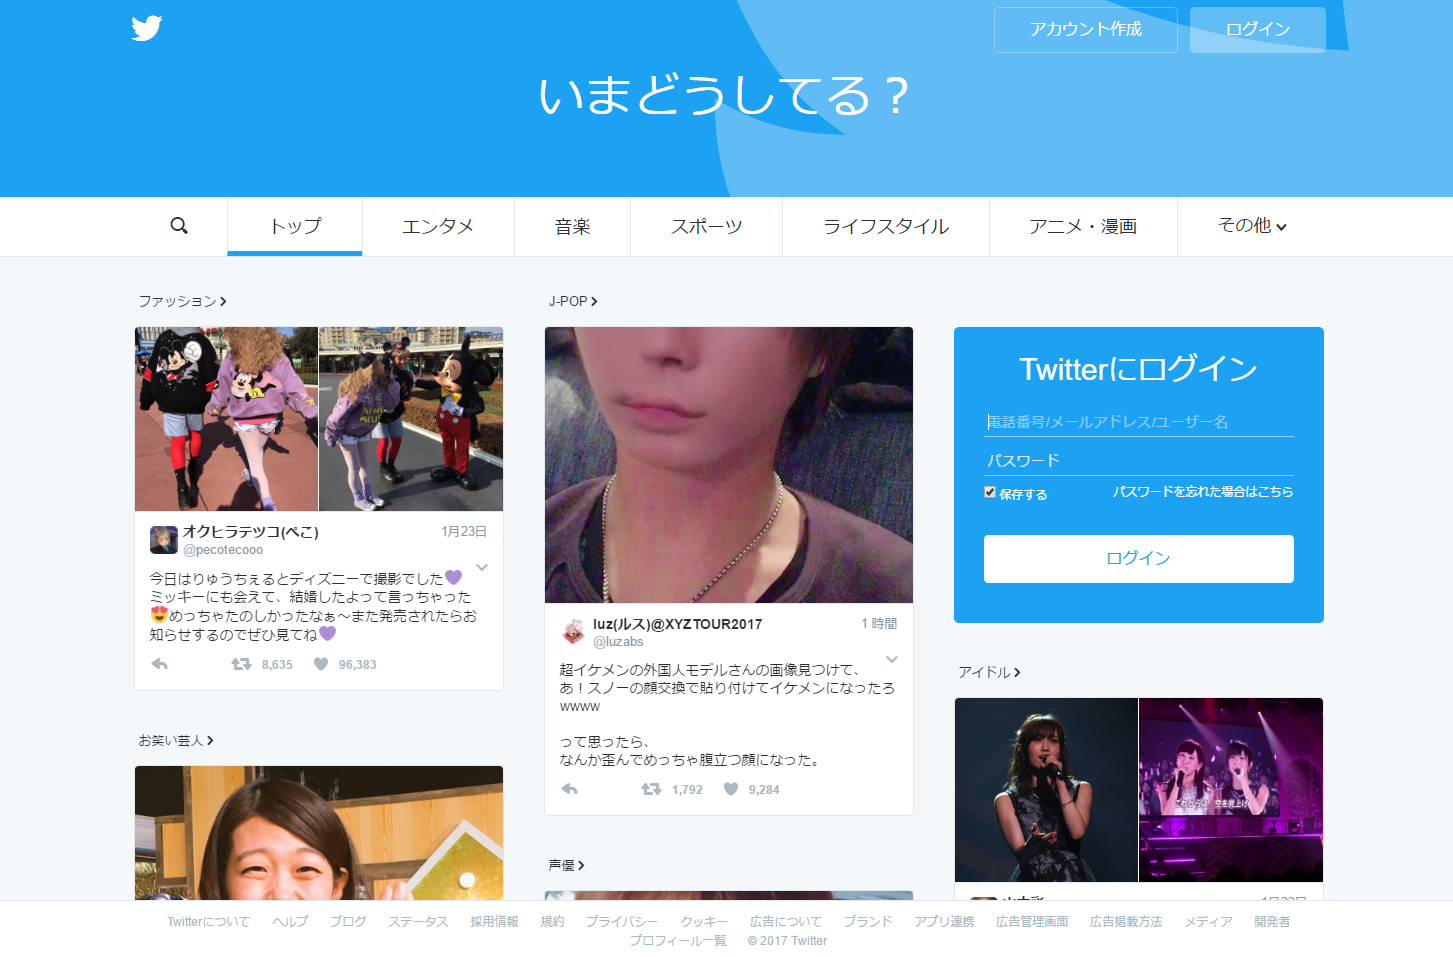
\includegraphics[width=15cm]{twitterhp.png}
\caption{twitterhp}\label{twitterhp}
\end{figure}
\clearpage
ニックネーム,電話番号又はメールアドレス,パスワードを入力してアカウント作成をクリックする.
\begin{figure}[htb]
\centering
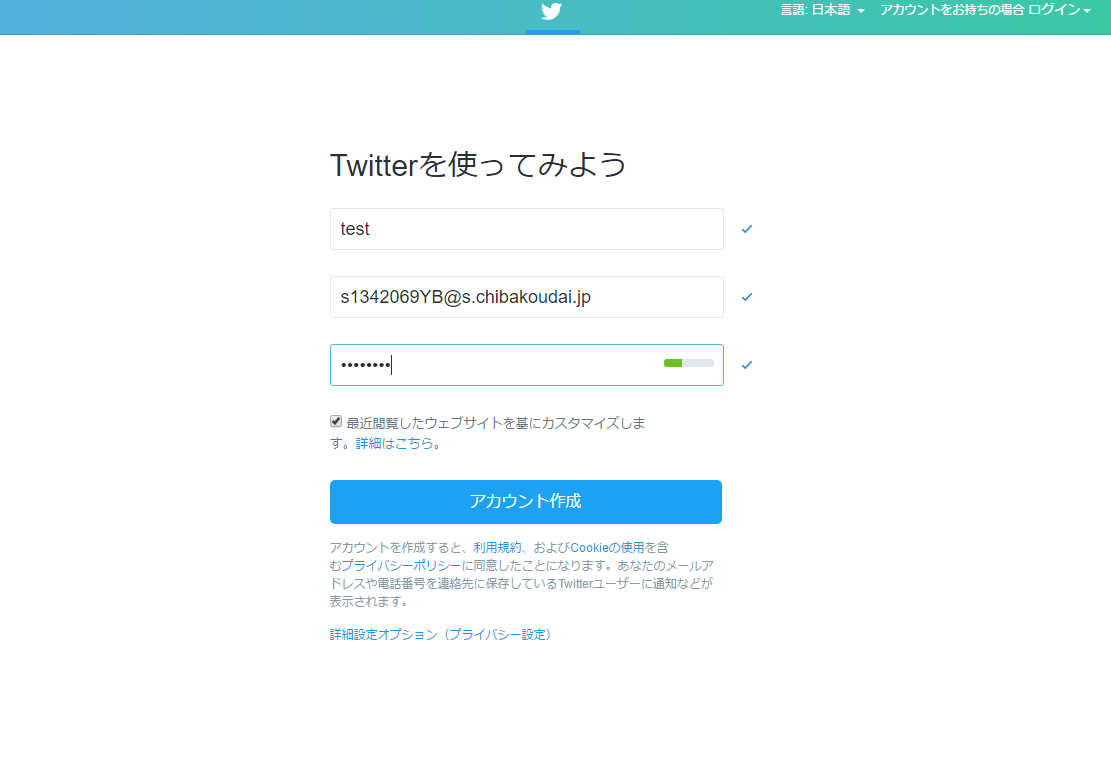
\includegraphics[width=15cm]{account.png}
\caption{account}\label{account}
\end{figure}
\clearpage
\subsection{開発者向けページ}
Twitter APIなどを利用する開発者向けのページ(https://dev.twitter.com/)へ行き,ページの下にある「Manage my apps」をクリックする.

\begin{figure}[htb]
\centering
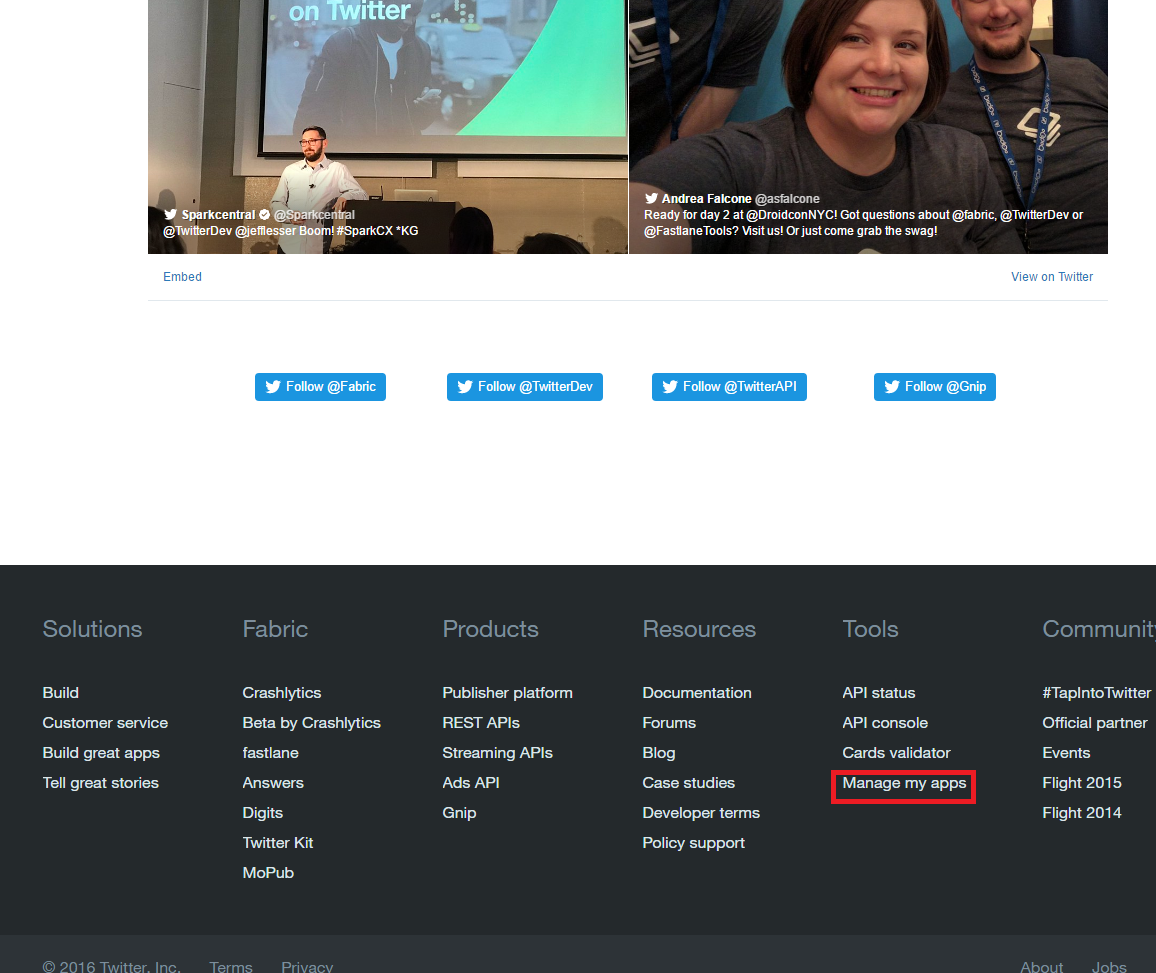
\includegraphics[width=13cm]{dev_twitter.png}
\caption{Twitterの開発者向けページ}\label{dev.twitter}
\end{figure}

\clearpage
「Please sign in with your Twitter Account to create and maintain Twitter Apps.」と出るのでsign inをクリックする.

\begin{figure}[htb]
\centering
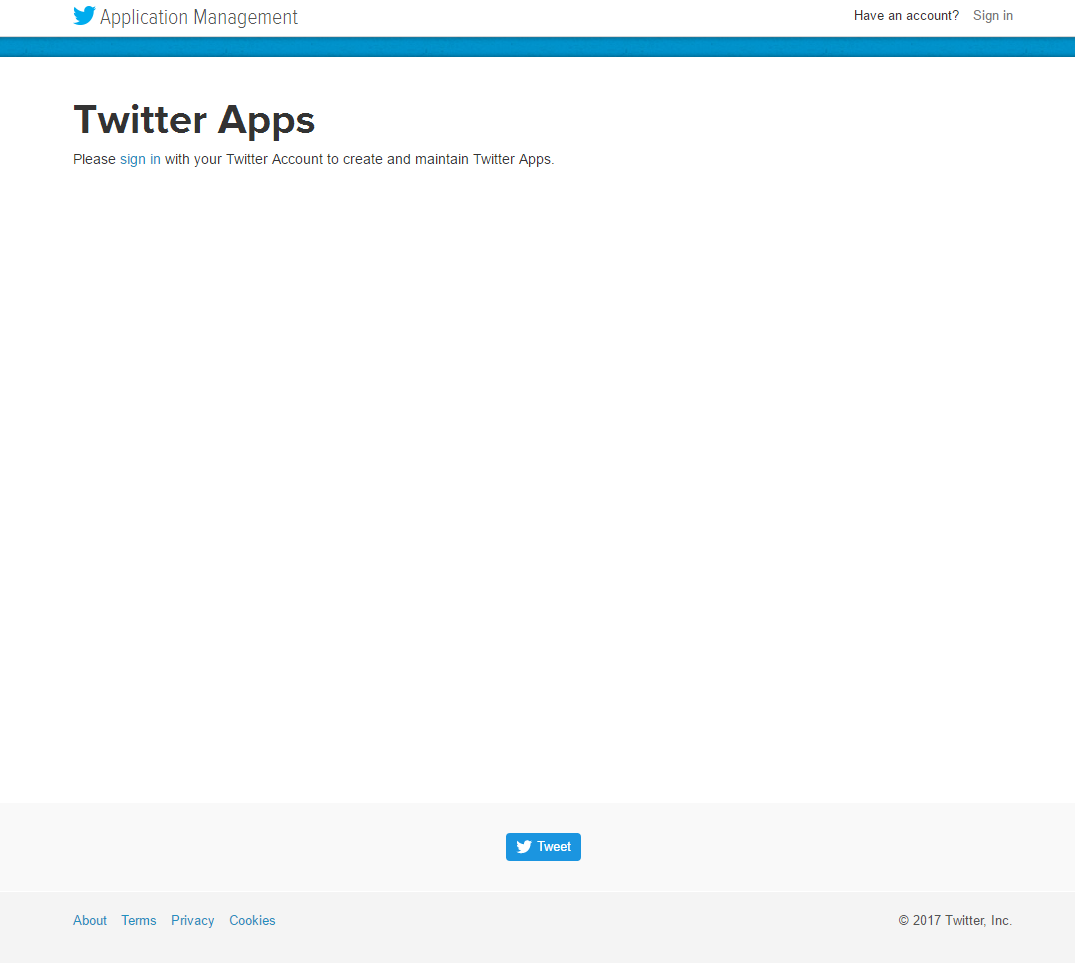
\includegraphics[width=13cm]{sign_in.png}
\caption{Twitter Apps}\label{sign_in}
\end{figure}
\clearpage
画面にTwitterに登録した電話番号/メールアドレス/ユーザー名のいずれかとパスワードを入力して下のログインをクリックする.

\begin{figure}[htb]
\centering
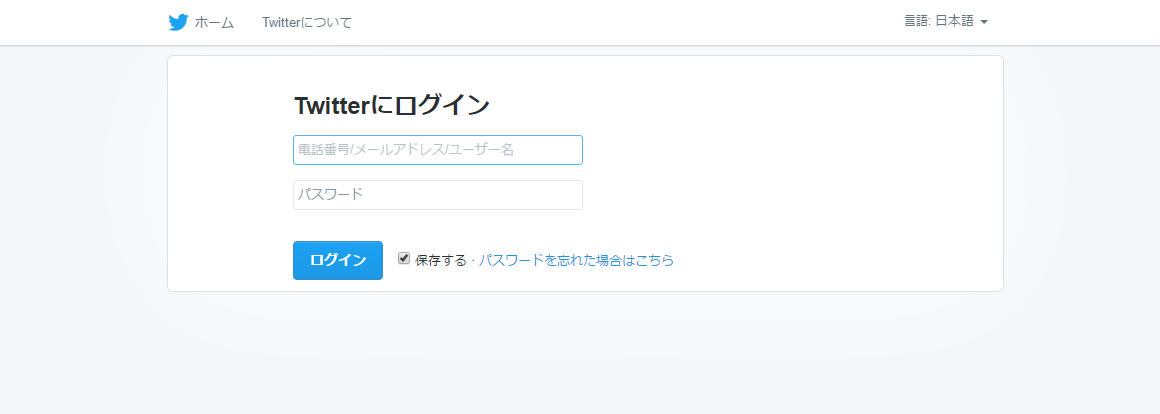
\includegraphics[width=13cm]{login.png}
\caption{ログイン画面}\label{login}
\end{figure}

「You don't currently have any Twitter Apps.」と表示されるので,その下にある「Create New App」をクリックする.

\begin{figure}[htb]
\centering
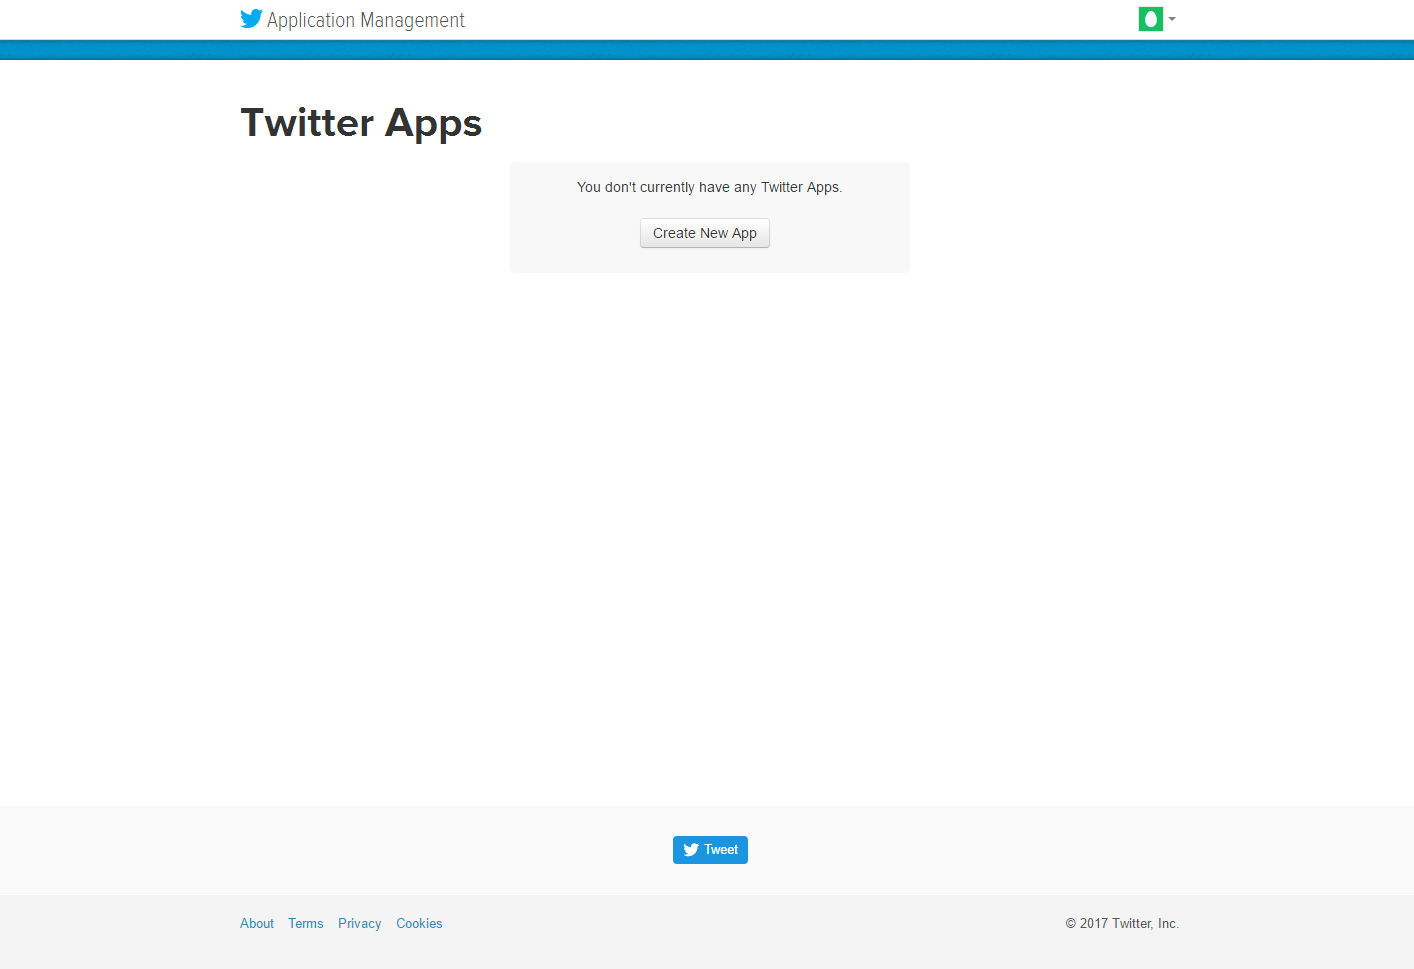
\includegraphics[width=13cm]{create_app.png}
\caption{create}\label{create_app}
\end{figure}
\clearpage
画面に「Name」,「Description」,「Website」をそれぞれ入力する.入力する内容は「Name」にはアプリケーションの名前,「Description」にはアプリケーションの説明,「Website」にはアプリケーションを動かすWebサイトのURL(本研究ではそういったWebサイトを使わないのでGitHubの自分のページのURLを入力した)を入力する.入力を終えたら「Yes,agree」にチェックを入れて,規約に同意し,「Create your Twitter application」をクリックするとアプリケーションが作成される.

\begin{figure}[htb]
\centering
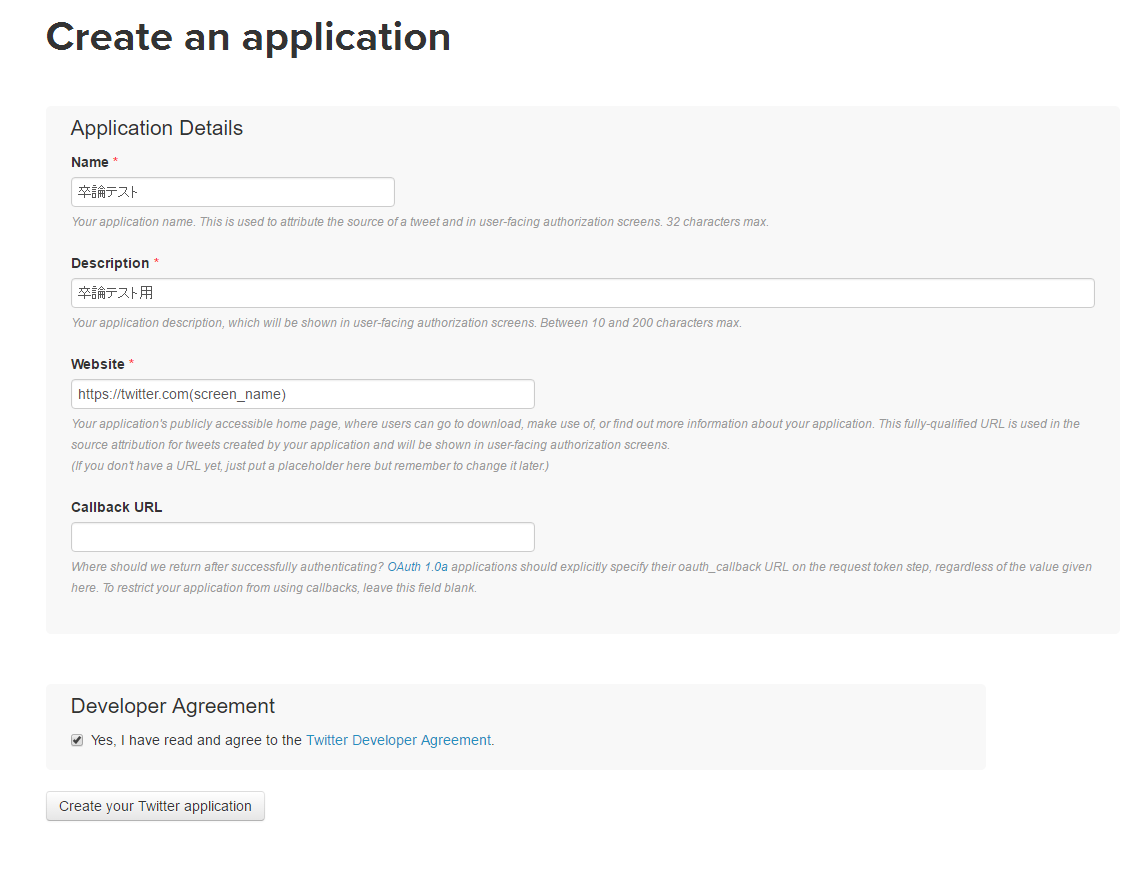
\includegraphics[width=13cm]{create.png}
\caption{create入力}\label{create}
\end{figure}
\clearpage

アプリケーションを作成したら,画面上部のKey and AccessTokensをクリックすると,「Consumer key」,「Consumer Sercret」,「Access Token」,「Access Token Secret」を確認できる.
\begin{figure}[htb]
\centering
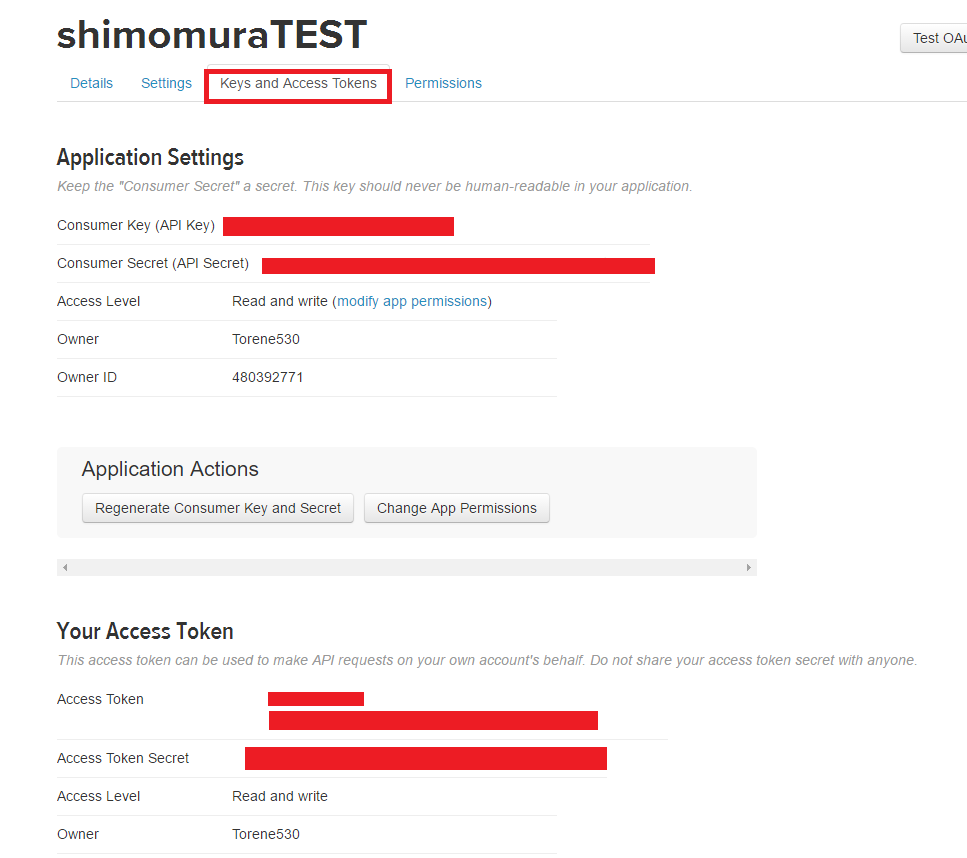
\includegraphics[width=13cm]{key.png}
\caption{アクセストークン}\label{key}
\end{figure}

\clearpage
\subsection{ランダムサンプリングの取得}
取得した「Consumer key」,「Consumer Sercret」,「Access Token」,「Access Token Secret」の情報を下記のプログラム(stream.py)に記入し,Ubuntuの端末から実行することによってランダムサンプリングを取得できる.
\begin{verbatim}
# -*- coding: utf-8 -*-

from tweepy.streaming import StreamListener
from tweepy import OAuthHandler
from tweepy import Stream

consumer_key = ""
consumer_secret = ""

access_token = ""
access_token_secret = ""

class StdOutListener(StreamListener):
    def on_data(self, data):
        if data.startswith("{"):
            print data
        return True
 
    def on_error(self, status):
        print status
 
if __name__ == '__main__':
    l = StdOutListener()
    auth = OAuthHandler(consumer_key, consumer_secret)
    auth.set_access_token(access_token, access_token_secret)
 
    stream = Stream(auth, l)
    #stream.filter( )#検索する場合
    stream.sample(languages =['ja'])#ツイートのランダムサンプリングを取得する場合
   # stream.userstream()#タイムラインを取得する場合
\end{verbatim}


\section{データベースの作成}

今回はTwitterのツイートを集めて管理する.収集したデータを簡単に検索、抽出できるようにデータベースを作成する.そのために以下のプログラムをUbuntuの端末から実行する.





\begin{verbatim}
 sudo apt-get install mysql-server mysql-client


 mysql -uroot -ppass

drop database if exists twitter;
create database twitter default charset=utf8;


grant all on twitter.* to test@localhost identified by 'pass';

use twitter;


drop table if exists users;
create table users (
  id bigint primary key,
  screenName varchar(100) not null,
  statuses int,
  friends int,
  followers int,
  lang varchar(10),
  profileImageUrl varchar(1000),
  rekognition text,
  index(lang),
  unique index(screenName)
);

desc users;


drop table if exists retweets;
create table retweets (
  id bigint primary key,
  retweet bigint not null,
  retweeted bigint not null,
  rcount int not null,
  fcount int not null,
  foreign key (retweet) references users (id),
  foreign key (retweeted) references users (id),
  unique index(retweet,retweeted)
);

desc retweets;


drop table if exists retweeters;
create table retweeters (
  id int auto_increment primary key,
  tweetId bigint not null,
  retweet bigint not null,
  foreign key (tweetId) references retweets (id),
  foreign key (retweet) references users (id)
);

desc retweeters;


drop table if exists friends;
create table friends (
  id int auto_increment primary key,
  user bigint not null,
  friend bigint not null,
  foreign key (user) references users (id),
  index(friend)
);

desc friends;


alter table users add friendsChecked boolean not null default false;
alter table users add index(friendsChecked);
alter table retweets add retweetersChecked boolean not null default false;
alter table retweets add index(retweetersChecked);


update users set friendsChecked = true where exists 
(select * from friends where friends.user=users.id);


update retweets set retweetersChecked = true where exists
 (select * from retweeters where retweeters.tweetId = retweets.id);


\end{verbatim}

1行目のsudo apt-get install mysql-server mysql-clientを入力すると,パスワードの入力を求められ,入力するとデータベースをインストールされる.

\clearpage
desc (テーブル名);を実行することでそのテーブルの構造を表示できる.
\begin{figure}[htb]
\centering
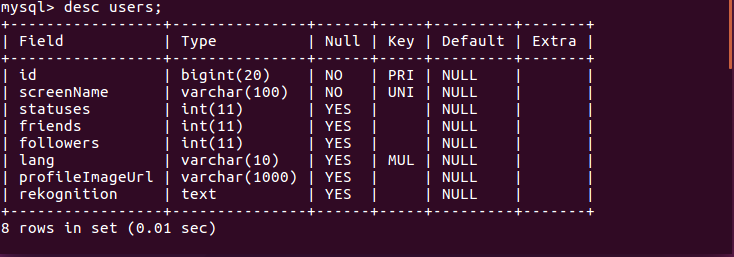
\includegraphics[width=13cm]{users.png}
\caption{users}\label{users}
\end{figure}

\begin{figure}[htb]
\centering
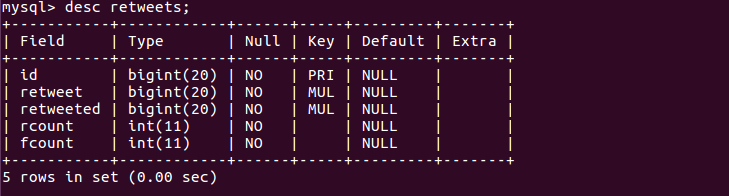
\includegraphics[width=13cm]{retweets.png}
\caption{retweets}\label{retweets}
\end{figure}
\newpage
\begin{figure}[htb]
\centering
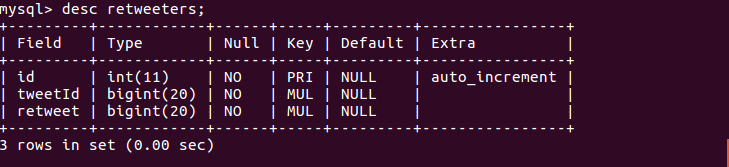
\includegraphics[width=13cm]{retweeters.png}
\caption{retweeters}\label{retweeters}
\end{figure}

\begin{figure}[htb]
\centering
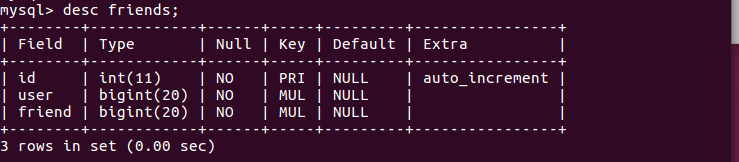
\includegraphics[width=13cm]{friends.png}
\caption{friends}\label{friends}
\end{figure}

\section{リツイートの記録}

\subsection{本章の構成}
本章ではリツイートを記録する方法を記述する.

\subsection{手順1}
streamingしたデータを標準出力に書き出す必要があり,そのために以下のプログラム(stream.py)をつくる.
その後,Ubuntuの端末に(python stream.py)を入力すると書き出される.
今回はツイートのランダムサンプリングを行う.
\begin{verbatim}

# -*- coding: utf-8 -*-

from tweepy.streaming import StreamListener
from tweepy import OAuthHandler
from tweepy import Stream

consumer_key = ""
consumer_secret = ""

access_token = ""
access_token_secret = ""

class StdOutListener(StreamListener):
    def on_data(self, data):
        if data.startswith("{"):
            print data
        return True
 
    def on_error(self, status):
        print status
 
if __name__ == '__main__':
    l = StdOutListener()
    auth = OAuthHandler(consumer_key, consumer_secret)
    auth.set_access_token(access_token, access_token_secret)
 
    stream = Stream(auth, l)
    #stream.filter( )#検索する場合
    stream.sample(languages =['ja'])#ツイートのランダムサンプリングを取得する場合
   # stream.userstream()#タイムラインを取得する場合

\end{verbatim}

\subsection{手順2}
手順1で標準出力したデータから,リツイートを抜き出し,データベースに記録するために以下のプログラム(retweets.py)を作る.その後Ubuntuの端末上で(python stream.py | python retweets.py)と入力すれば,リツイートを抜き出し,データベースに記録される.

\begin{verbatim}
# -*- coding: utf-8 -*-
#!/usr/bin/env python
import sys, json
from pprint import pprint

def extractUserProfile(user):
  id = user['id_str']
  screenName = user['screen_name']
  statuses = user['statuses_count']
  friends = user['friends_count']
  followers = user['followers_count']
  lang = user['lang']
  profileImage = user['profile_image_url'].replace('_normal.', '.')#プロフィール画像(オリジナルサイズ)
  sys.stdout.write("insert into users 
  (id,screenName,statuses,friends,followers,lang,profileImageUrl)
   values (%s,'%s',%d,%d,%d,'%s','%s');\n"
    % (id, screenName, statuses, friends, followers, lang, profileImage))
  return id

for line in sys.stdin:
  try:
    tweet = json.loads(line)
    #pprint(tweet)
    if 'retweeted_status' in tweet:
      #pprint(tweet)#内容確認(これを有効にして「| less」で実行する)
      
      retweet = extractUserProfile(tweet['user'])#リツイートした人
      
      retweetedStatus = tweet['retweeted_status']
      tweet = retweetedStatus['id_str']#ツイートID
      rcount = retweetedStatus['retweet_count']#ツイート回数
      fcount = retweetedStatus['favorite_count']#ファボ数
      retweeted = extractUserProfile(retweetedStatus['user'])#リツイートされた人

      sys.stdout.write("insert into retweets (id,retweet,retweeted,rcount,fcount) 
      values (%s,%s,%s,%d,%d);\n" % (tweet, retweet, retweeted, rcount, fcount))
      sys.stdout.flush()
  except ValueError:
    pass
\end{verbatim}

\subsection{手順3}
データベースに記録する.

Ubuntuの端末上で以下のコマンドを実行しデータベースに記録する.
python stream.py | python retweets.py | mysql -utest -ppass --force twitter
--forceをつけることにより,集めたデータに重複が出た場合のエラーが出ても止まらないようになる.

\clearpage

Ubuntuの端末に以下のコマンドを実行するとデータベースに記録したリツイートのデータ確認できる.
select * from retweets;

\begin{figure}[htb]
\centering
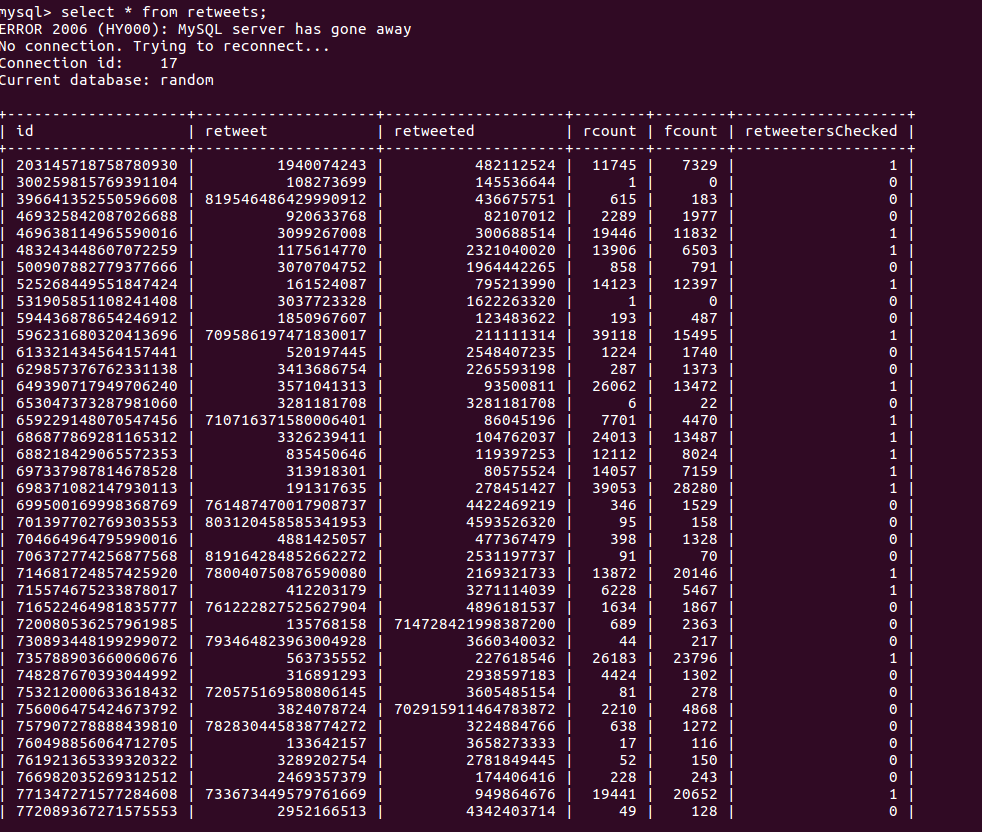
\includegraphics[width=13cm]{table_retweets.png}
\caption{retweetsテーブル}\label{table_retweets}
\end{figure}

\newpage

\section{リツイートした人がフォローしている人の取得}

\subsection{本章の構成}
本章ではリツイートした人がフォローしている人の取得について記述する.

\subsection{リツイートした人がフォローしている人数の取得}
指定したIDのユーザがフォローしている人数を取得するために以下のプログラム(friends.py)を作成する.

\begin{verbatim}
 -*- coding: utf-8 -*-

import tweepy
import json
import sys
from pprint import pprint
from auth import api

for line in sys.stdin:
  userId = line.rstrip()
  sys.stderr.write("checking friends of %s...\n" % userId)
  
  #フレンドを調べたことを記録する。
  sys.stdout.write("update users set friendChecked=true where id=%s;\n" % (userId))
  
  try:
    friends = api.friends_ids(userId)
    for friendId in friends:
      sys.stdout.write("insert into friends (user,friend)
       values (%s,%s);\n" % (userId, friendId))
    sys.stdout.flush()
  except:
    pass

\end{verbatim}

Ubuntuの端末上で以下のコマンドを実行すると,指定したIDのユーザがフォローしている人を取得する.
\newline
echo XXXXX | python friends.py | mysql -utest -ppass --force twitter (XXXXXはユーザID)
また,usersに実在するIDを使わなければ外部キーエラーになるのでデータベースに登録したデータを使う.
\newline
データベースから未調査のリツイートを取得する場合は以下のコマンドを端末上で実行する.
\newline

echo "select retweet from retweets join users on users.id=retweets.retweet where users.friendsChecked=false limit 1;" | mysql -utest -ppass --skip-column-names twitter | python friends.py | mysql -utest -ppass --force twitter
\newline

Ubuntuの端末に以下のコマンドを実行するとデータベースに記録したリツイートのデータ確認できる.
select * from friends;
\newline
\begin{figure}[htb]
\centering
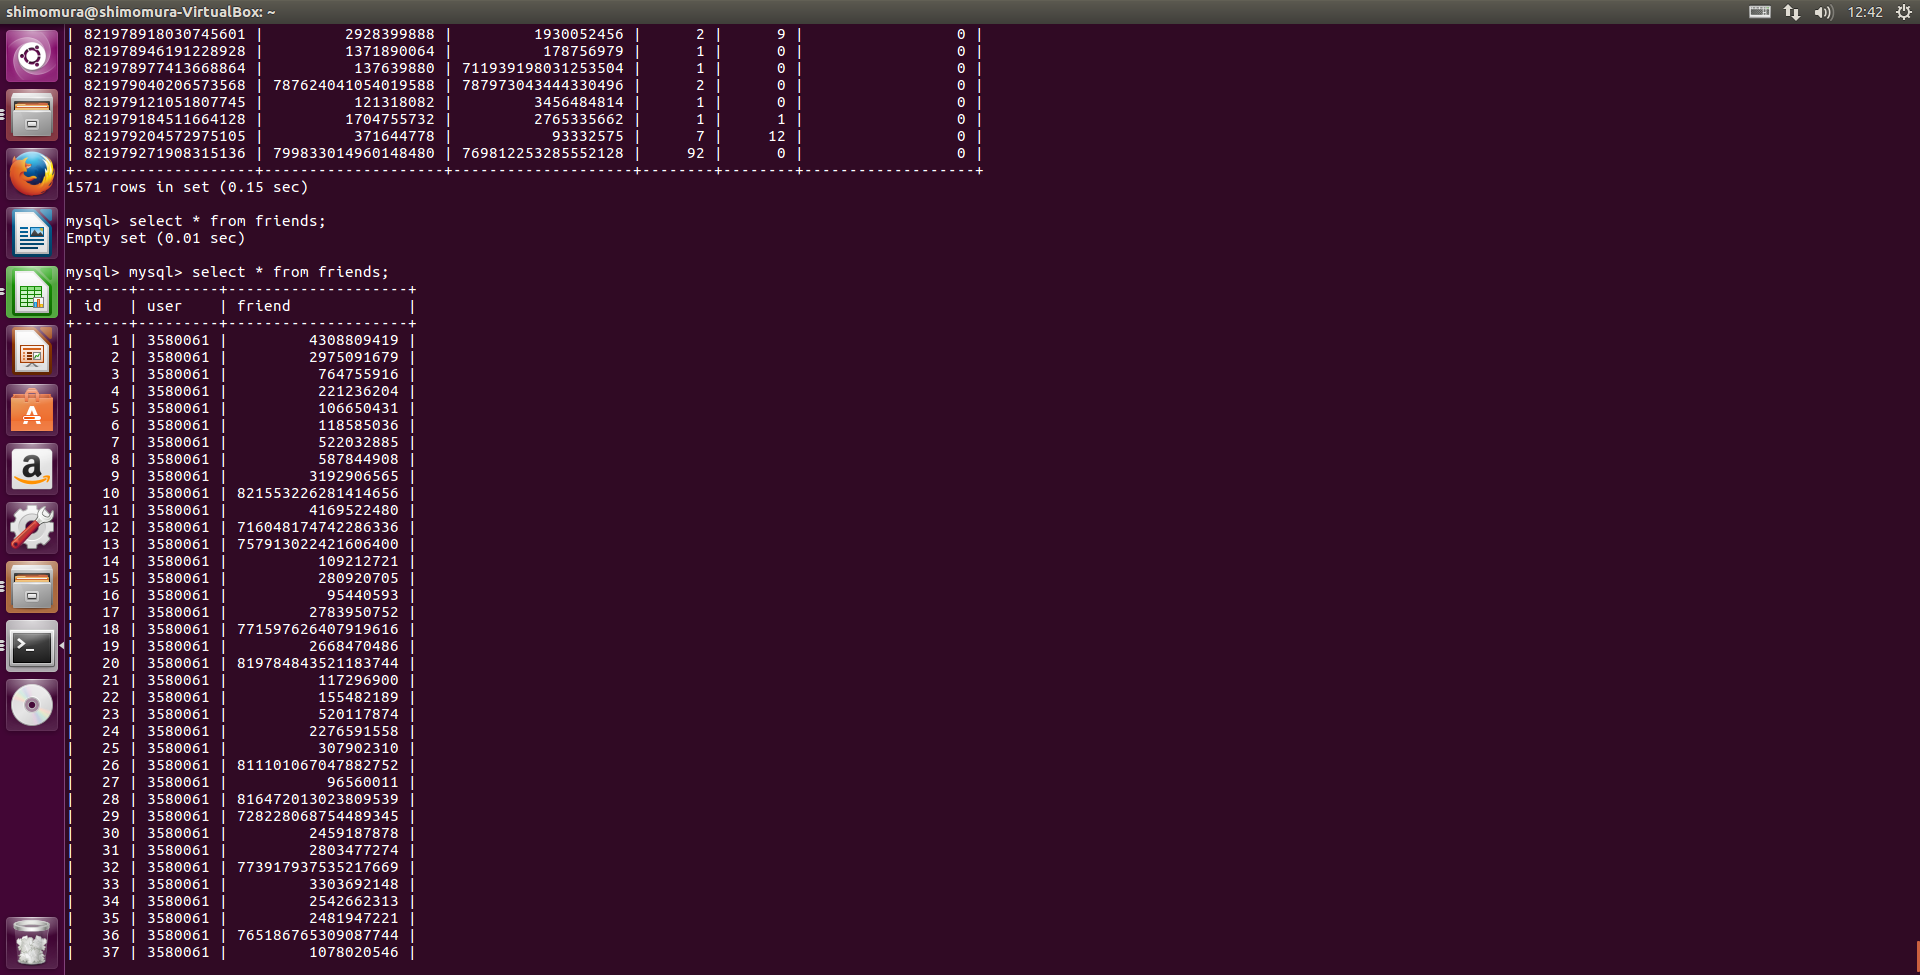
\includegraphics[width=13cm]{table_friends.png}
\caption{friendsテーブル}\label{table_friends}
\end{figure}

\newpage

\subsection{本章の構成}
本章ではリツイートした人のリストの取得について記述する.

\subsection{リツイートした人がフォローしている人数の取得}
指定したIDのツイートをリツイートした人を取得するために(以下のプログラム(retweeters.py)を作成する.

\begin{verbatim}
 # -*- coding: utf-8 -*-

import tweepy
import json
import sys
from pprint import pprint
from auth import api

for line in sys.stdin:
  tweetId = line.rstrip()
  sys.stderr.write("checking retweeters of %s...\n" % tweetId)
  
  #リツイートした人を調べたことを記録する。
  sys.stdout.write
("update retweets set retweetersChecked=true where id=%s;\n" % (tweetId))
  
  try:
    retweeters = api.retweets(tweetId, 100)
    for t in retweeters:
      #このオブジェクトの中身がわかりにくい。(PyDevのデバッガで調べた。)
      user = t.user
      userId = user.id_str
      screenName = user.screen_name
      statuses = user.statuses_count
      friends = user.friends_count
      followers = user.followers_count
      profileImage = user.profile_image_url.replace('_normal.', '.')#プロフィール画像(オリジナルサイズ)
      
      sys.stdout.write
("insert into users (id,screenName,statuses,friends,followers,profileImageUrl)
values (%s,'%s',%d,%d,%d,'%s');\n" %
 (userId, screenName, statuses, friends, followers, profileImage))
#これは重複エラーになるはず
      sys.stdout.write("insert into retweeters (tweetId,retweet) 
values (%s,%s);\n" % (tweetId, userId))
    sys.stdout.flush()
  except:
    pass

\end{verbatim}

Ubuntuの端末上で以下のコマンドを実行すると,指定したIDのツイートをリツイートした人を取得する.


echo 557560378758942720 | python retweeters.py | mysql -utest -ppass --force twitter
また,テーブルretweetsの中に存在するIDを使わないと外部キーエラーになるのでデータベースに登録したデータを使う.
\newline
データベースから未調査のリツイートを取得する場合は以下のコマンドを端末上で実行する.
\newline
echo "select id from retweets where retweetersChecked=false limit 1;" | mysql -utest -ppass --skip-column-names twitter | python retweeters.py | mysql -utest -ppass --force twitter
\newline
\newpage
Ubuntuの端末に以下のコマンドを実行するとデータベースに記録したリツイートのデータ確認できる.
select * from retweeters;
\newline
\begin{figure}[htb]
\centering
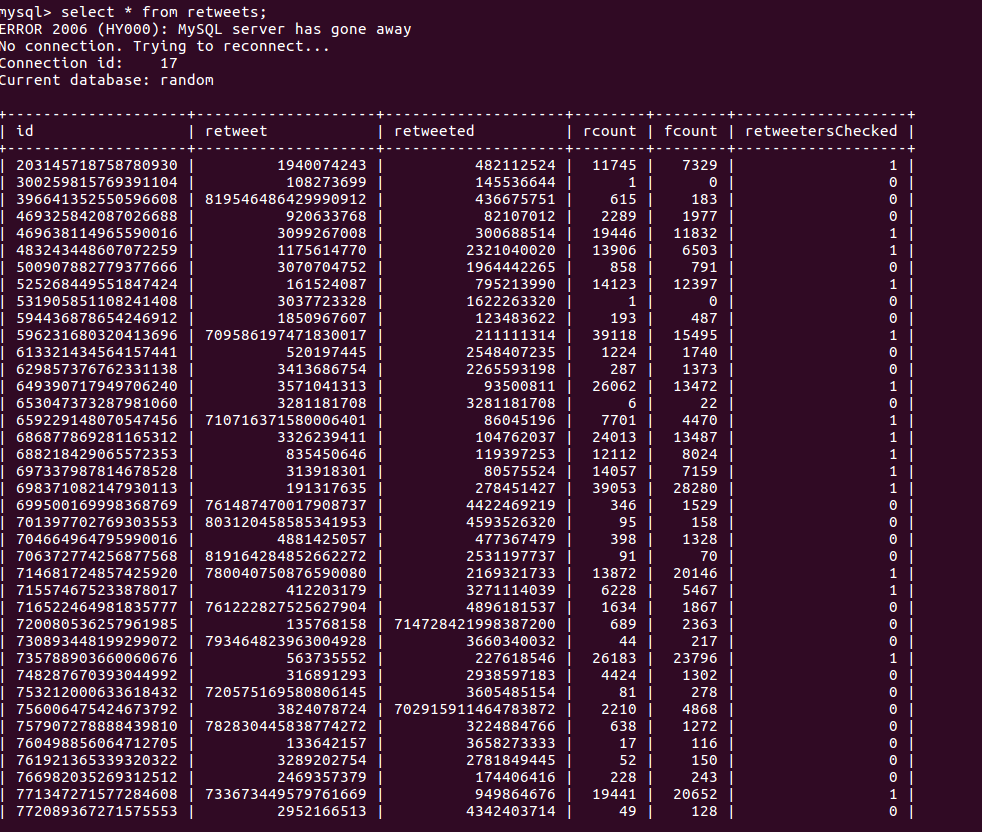
\includegraphics[width=13cm]{table_retweets.png}
\caption{retweetsテーブル}\label{table_retweets}
\end{figure}



\chapter{結果}
\subsection{研究結果}
本章では,研究結果を記述する.
   

\subsection{取得したデータが入ったテーブルのエクスポート}

Ubuntu上でselect * into outfile '/var/lib/mysql-files/〇〇〇.csv' from 〇〇〇;(○○○にはテーブルの名前を入力)を実行し,テーブルの情報CSVでエクスポートし,Excelにインポートする.

\begin{figure}[htb]
\centering
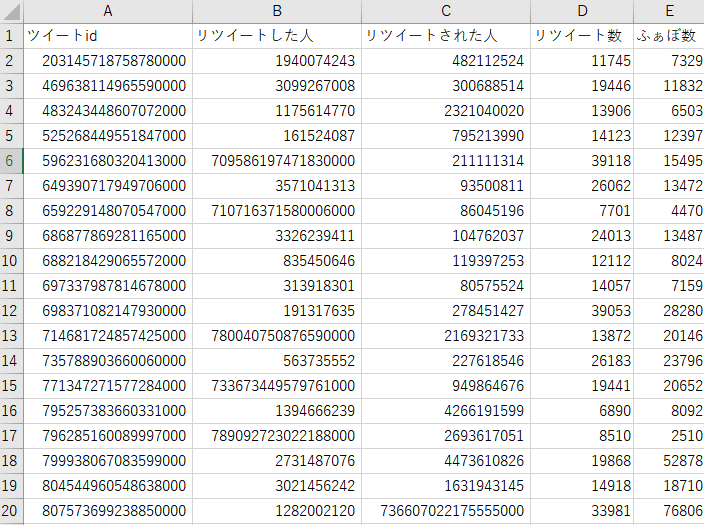
\includegraphics[width=10cm]{excel_retweets.png}
\caption{エクセルretweets}\label{excel_retweets}
\end{figure}

\clearpage

\begin{figure}[htb]
\centering
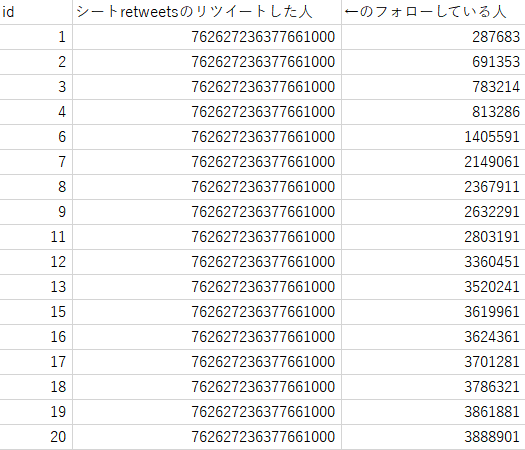
\includegraphics[width=10cm]{excel_friends.png}
\caption{エクセルfriends}\label{excel_friends}
\end{figure}
\clearpage
\begin{figure}[htb]
\centering
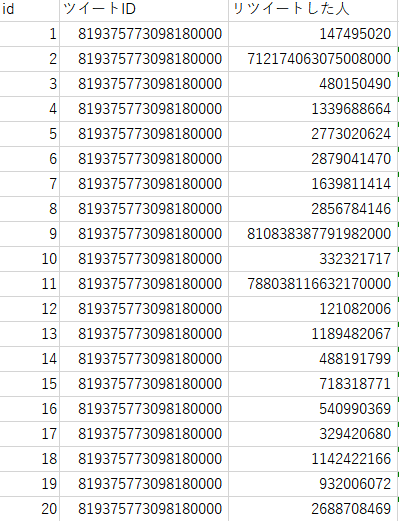
\includegraphics[width=10cm]{excel_retweeters.png}
\caption{エクセルretweeters}\label{excel_retweeters}
\end{figure}
\clearpage

炎上ツイートの定義をリツイート数が5000以上されたものとし,ランダムサンプリングしたツイートの中からリツイート数が5000以上ものを100件取得した.その100件のツイートをリツイートしているユーザーを取得した結果,2件以上リツイートしたユーザーは366001人中146人で,ツイートした人をフォローしている人は245人だった.
\clearpage

\chapter{考察}
\subsection{本省の構成}
本章では,考察を記述する.
\subsection{考察}
5000以上リツイートされたものを炎上としたとき,炎上ツイートした人をフォローしている人が炎上を拡散することは少なく,フォローをしていない人の方が炎上を拡散していると考えられる.

\clearpage

\chapter{結論}
\subsection{本省の構成}
本章では,結論を記述する.
\subsection{結論}
本研究では,リツイートした人とリツイートされた人の関係性を調べることができた.炎上したツイートは消されることが多くデータを収集するのが艱難なので,どのようにデータを収集するのかが今後の課題である.
\bibliographystyle{junsrt}
\bibliography{biblio}%「biblio.bib」というファイルが必要.

\end{document}

